\documentclass[xcolor=dvipsnames,10pt,aspectratio=169]{beamer}
%\documentclass[xcolor=dvipsnames,10pt]{beamer}
\usepackage{etex}
\usepackage{pgf,pgfarrows,pgfnodes,pgfautomata,pgfheaps,pgfshade}
\usepackage[absolute,overlay]{textpos} 
%\usepackage{algorithm}
\usepackage{amsmath,amssymb}
\usepackage[utf8]{inputenc} 
\usepackage{colortbl}
\usepackage{graphicx} 
\usepackage[brazil]{babel}
\usepackage{tabularx} 
\usepackage{multirow}
\usepackage{booktabs}
\usepackage{listings}
%\usepackage{multimedia}
\usepackage{animate}
\usepackage{xcolor}
\usepackage{array}
\usepackage{longtable}
\usepackage{makecell}
\usepackage{caption}
\usetheme{Madrid} 
\usepackage{amsmath}
\usepackage{movie15}


\lstset{ %
%	backgroundcolor=\color{white},   % choose the background color; you must add \usepackage{color} or \usepackage{xcolor}
%	basicstyle=\footnotesize,        % the size of the fonts that are used for the code
	basicstyle=\scriptsize,        % the size of the fonts that are used for the code
	breakatwhitespace=false,         % sets if automatic breaks should only happen at whitespace
	breaklines=true,                 % sets automatic line breaking
	captionpos=t,                    % sets the caption-position to bottom
	commentstyle=\color{mygreen},    % comment style
	deletekeywords={...},            % if you want to delete keywords from the given language
	escapeinside={\%*}{*)},          % if you want to add LaTeX within your code
	extendedchars=true,              % lets you use non-ASCII characters; for 8-bits encodings only, does not work with UTF-8
%	frame=single,                    % adds a frame around the code
	keepspaces=true,                 % keeps spaces in text, useful for keeping indentation of code (possibly needs columns=flexible)
	keywordstyle=\color{blue},       % keyword style
%	language=make,                 % the language of the code
	morekeywords={*,...},            % if you want to add more keywords to the set
%	numbers=left,                    % where to put the line-numbers; possible values are (none, left, right)
%	numbersep=5pt,                   % how far the line-numbers are from the code
	numberstyle=\tiny\color{mygray}, % the style that is used for the line-numbers
	rulecolor=\color{black},         % if not set, the frame-color may be changed on line-breaks within not-black text (e.g. comments (green here))
	showspaces=false,                % show spaces everywhere adding particular underscores; it overrides 'showstringspaces'
	showstringspaces=false,          % underline spaces within strings only
	showtabs=false,                  % show tabs within strings adding particular underscores
	stepnumber=2,                    % the step between two line-numbers. If it's 1, each line will be numbered
}

\definecolor{mygreen}{rgb}{0,0.6,0}
\definecolor{mygray}{rgb}{0.5,0.5,0.5}
\definecolor{mymauve}{rgb}{0.58,0,0.82}

\usecolortheme{beaver}
\newcommand{\ul}{\underline}
\setbeamertemplate{footline}{\scriptsize{\vspace*{0.3cm}\hspace*{15cm}\insertframenumber\,/\,\inserttotalframenumber}}
\setbeamertemplate{caption}[numbered]
\setbeamerfont{caption}{size=\fontsize{8}{5}}

\setbeamercolor{block title}{	bg=Sepia , fg = White}
\setbeamercolor{block body}{bg=Brown!15, fg=Sepia }
\setbeamercolor{item projected}{bg=Sepia, fg=White}
\setbeamercolor{number projected}{bg = Black}

%declara as imagens usadas no layout do slide
\pgfdeclareimage[height=0.8cm]{mflab}{figuras/logo_mflab_transparente.png}
\pgfdeclareimage[height=1.0cm]{logoufu}{figuras/logo_ufu.jpg}
\pgfdeclareimage[height=1.0cm]{petro}{figuras/petrobras_2.png}

%posiciona o logotipo do MFLab
\setlength{\TPHorizModule}{1mm}
\setlength{\TPVertModule}{1mm}
\newcommand{\placelogomflab} 
{ 
	\begin{textblock}{13}(150.0,0.0)
		\pgfuseimage{mflab} 
	\end{textblock} 
	
% 	\begin{textblock}{13}(128.0,1.0)
% 		\pgfuseimage{logoufu} 
% 	\end{textblock} 
	
	\begin{textblock}{13}(150.0,70.0)
		\pgfuseimage{petro} 
	\end{textblock} 
}
%posiciona o logotipo do MFLab
\setlength{\TPHorizModule}{1mm}
\setlength{\TPVertModule}{1mm}
\newcommand{\placelogo} 
{ 
	\begin{textblock}{13}(150.0,0.0)
		\pgfuseimage{mflab} 
	\end{textblock} 
	
% 	\begin{textblock}{13}(128.0,1.0)
% 		\pgfuseimage{logoufu} 
% 	\end{textblock} 
	
	\begin{textblock}{13}(0.0,80.0)
		\pgfuseimage{petro} 
	\end{textblock} 
}

% \setlength{\TPHorizModule}{1mm}
% \setlength{\TPVertModule}{1mm}
% \newcommand{\placelogomflab_titulo} 
% { 
% 	\begin{textblock}{13}(150.0,0.0)
% 		\pgfuseimage{mflab} 
% 	\end{textblock} 
% 	
% 	\begin{textblock}{13}(0.0,0.0)
% 		\pgfuseimage{lmest} 
% 	\end{textblock} 
% 	
% % 	\begin{textblock}{13}(128.0,1.0)
% % 		\pgfuseimage{logoufu} 
% % 	\end{textblock} 
% 	
% 	\begin{textblock}{13}(75.0,80.0)
% 		\pgfuseimage{petro} 
% 	\end{textblock} 
% }



%insere o logotipo da ufu em todos os slides
% \logo{
\includegraphics[height=0.8cm]{figuras/layout_slide/petrobras.png}}

\title{Análise teórica de escoamentos de Poiseuille planos com efeitos térmicos: ajuste do número de Prandtl turbulento e do número de Cebeci}

\author{ Felipe J. O. Ribeiro \\ \and \\ Orientador: Prof. Dr. Aristeu da Silveira Neto}

%\date{\tiny{02 de dezembro de 2015}}
\date{\tiny{\today}}
% \newcolumntype{M}[1]{>{\raggedright\arraybackslash}b{#1}}
% \newcolumntype{N}{@{}m{0pt}@{}}	
% \newcolumntype{M}{>{\begin{minipage}[b]{3cm}\raggedright{}}c<{\end{minipage}\minrowheight}}
% \setlength\extrarowheight{5pt}
\newcolumntype{C}[1]{>{\centering\let\newline\\\arraybackslash\hspace{0pt}}m{#1}}


\begin{document}

	\begin{frame}\placelogomflab
		\frametitle 
		{ \vfill
			\centering
			{
			\small{Universidade Federal de Uberlândia}\\
%			\small{Programa de Pós-Graduação em Engenharia Mecânica}\\
			\small{Laboratório de Mecânica dos Fluidos}\\
			}
		}
		\maketitle
	\end{frame}

	\section<presentation>*{Sumário}
	
		\begin{frame}
			\frametitle{Sumário}\placelogomflab 
			{\scriptsize \tableofcontents}
		\end{frame}

		\AtBeginSection[]
		{
		 \begin{frame}<beamer>
		  \frametitle{Sumário}\placelogomflab 
		  {\scriptsize \tableofcontents[current,currentsection]}
		 \end{frame}
		}

		\AtBeginSubsection[]
		{
		 \begin{frame}<beamer>
		  \frametitle{Sumário}\placelogomflab 
		  {\scriptsize \tableofcontents[current,currentsubsection]}
		 \end{frame}
		}


	\section{Introdução}
	
	
	
	
	
	
		\begin{frame}
		\frametitle{Análise térmica em escoamentos turbulentos de Poiseuille}
			\begin{minipage}[h!]{0.49\textwidth}
			$\bullet$ O estudo do comportamento térmico de escoamentos é de suma importância ao desenvolvimento científico atual. A medida que o maquinário industrial é aperfeiçoado, também cresce o consumo energético no mundo. Grande parte deste custo surge das transformações energéticas dentro do sistema, em sua maioria, resultando em manifestações térmicas. Assim surge uma grande necessidade de mecanismos de gerenciamento térmico. Como a difusão é um processo muito lento, o meio mais utilizado para se resfriar maquinários industriais é o advectivo, onde uma interface fluido-estrutura carrega energia térmica para fora do sistema. Estudar estes fenômenos é essencial para que hajam cada vez máquinas mais eficientes, assim assegurando um desenvolvimento sustentável. 
		\end{minipage}
		\begin{minipage}[h!]{0.49\textwidth}
			\begin{figure}[h!]
				\centering
				
\includegraphics[trim = {1.7cm 2cm 0 1cm}, clip , angle=0, scale=0.60]{turbulence}
				\caption{Temperatura e turbulência.}
			\end{figure}
		\end{minipage}
		\end{frame}





	\section{Modelo físico}
	
	
	
	
	
		\begin{frame}
			\frametitle{Escoamento de Poiseuille plano}
			$\bullet$ O problema foi definido como um escoamento de canal, com somente uma dimensão finita no eixo $y$. \\
			$\bullet$ As condições de contorno foram determinadas como duas placas infinitas em um regime de fluxo térmico constante.\\
			$\bullet$ Um gradiente de pressão constante foi imposto no eixo $x$.\\
			$\bullet$ Foi proposta uma auto similaridade dinâmica e térmica no eixo $z$, resultando em uma análise dinâmica unidimensional e térmica bidimensional (Fig.\ref{figure.1}). \\
			$\bullet$ Foram considerados escoamentos incompressíveis de fluido newtoniano em regime turbulento.\\
			\begin{minipage}[h!]{0.3\textwidth}
				\begin{equation*}
				 \frac{\partial T }{\partial z} = 0.
				\end{equation*}
				\begin{equation*}
				\frac{\partial u }{\partial z} = 0.
				\end{equation*}
				\begin{equation*}
				\frac{\partial u }{\partial x} = 0.
				\end{equation*}
			\end{minipage}
			\begin{minipage}[h!]{0.5\textwidth}
			\begin{figure}[h!]
				\centering
				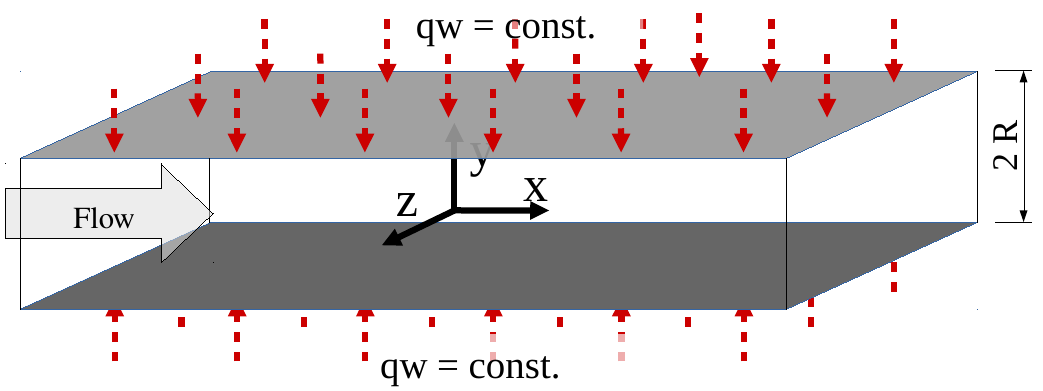
\includegraphics[angle=0, scale=0.30]{figure1}
				\caption{Definições geométricas e condições de contorno do sistema.}
				\label{figure.1}
			\end{figure}
			\end{minipage}
			\\
		\end{frame}
	
	

	
	\section{Modelo matemático diferencial}
	
	
	
	
		
		\begin{frame}
		\frametitle{Equações do movimento}
		$\bullet$ Para modelar diferencialmente a velocidade do fluido, foram utilizadas a equação da continuidade e a equação de Navier-Stokes para a velocidade no eixo de interesse.
		\begin{equation}
		\frac{\partial u}{\partial t} + \frac{\partial u^2}{\partial x} + \frac{\partial uv}{\partial y} + \frac{\partial uw}{\partial z} = - \frac{1}{\rho} \frac{\partial {p}}{\partial x} + \nu \left( \frac{\partial^2 u}{\partial x^2} + \frac{\partial^2 u}{\partial y^2} + \frac{\partial^2 u}{\partial z^2}   \right)
		\end{equation}
		\begin{equation}
		\frac{\partial \rho}{\partial t} +  \frac{\partial (\rho u)}{\partial x} + \frac{\partial (\rho v)}{\partial y} + \frac{\partial (\rho w)}{\partial z} = 0
		\end{equation}
		Para o desenvolvimento da equação da energia em uma instancia convectiva foi necessário o desenvolvimento do perfil cinético do sistema.
		\end{frame}

		



		\begin{frame}
		\frametitle{Equação do balanço da energia térmica}
		$\bullet$ Foi utilizada a equação da energia térmica.
		\begin{equation}
		\frac{\partial T}{\partial t} + {\frac{\partial{}}{\partial{x}} (uT)} + {\frac{\partial{}}{\partial{y}} (vT)} + {\frac{\partial{}}{\partial{z}} (wT)}
		=
		{\frac{\partial{}}{\partial{x}}} \left(\alpha {\frac{\partial{T}}{\partial{x}}} \right) +
		{\frac{\partial{}}{\partial{y}}} \left(\alpha {\frac{\partial{T}}{\partial{y}}} \right) +
		{\frac{\partial{}}{\partial{z}}} \left(\alpha {\frac{\partial{T}}{\partial{z}}} \right) .
		\end{equation}
		$ $
		$\bullet$ Sendo necessária esta definição para adimensionalização.
		\begin{equation}\label{c_h_e}
		q_{conv.} = \dot{m} C_p \Delta T_m.
		\end{equation}
		$ $
		Com estas construções matemáticas foi possível se iniciar o desenvolvimento diferencial.
		\end{frame}




		
		
		\begin{frame}
			\frametitle{Princípio dos valores médios}
			$\bullet$ Para se prosseguir com as simplificações das equações diferenciais foi necessário se utilizar os conceitos de valores médios. Tal consideração implica no uso do modelo RANS. (Reynolds Averaged Navier Stokes)
			\\
			\begin{minipage}[h!]{0.45\textwidth}
				\begin{equation*}
				\label{ola}
				\text{Simplificação}=
				\begin{cases}
				\overline{f}({x})=\frac{1}{t_f - t_i} \int_{t_i}^{t_f} f({x} , t) dt.      & \quad  \\
				f({x} , t) = \overline{f}({x}) + f^\prime ({x} ,t) . & \quad   \\
				\overline{f^\prime ({x} ,t)} = 0 . & \quad   \\
				\overline{\overline{f({x})}} = \overline{f({x})} . & \quad   \\
				\overline{f^\prime ({x} ,t)\overline{f({x})}} = 0 .& \quad   \\
				\overline{f^\prime ({x} ,t)g^\prime ({x} ,t)} \neq 0 . & \quad   \\
				\overline{  \overline{g({x})} \ \overline{f({x})}  } = {\overline{g({x})}} \ {\overline{f({x})}} . & \quad   \\
				\end{cases}
				\end{equation*}
			\end{minipage}\hfill
			\begin{minipage}[h!]{0.45\textwidth}
				\begin{figure}
					\centering
					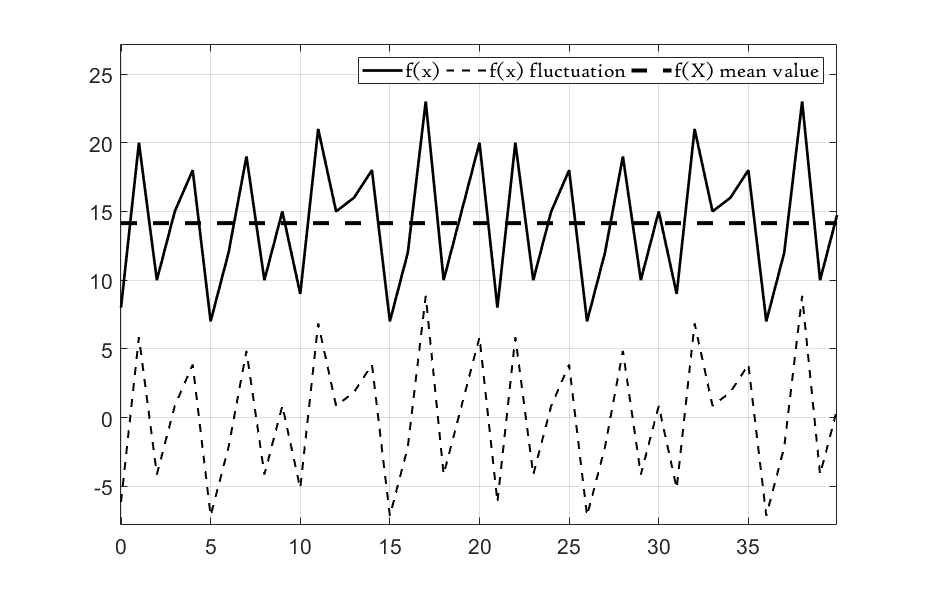
\includegraphics[angle=0, scale=0.3]{medios}
					\caption{Representação gráfica do conceito.}
					\label{medios}
				\end{figure}
			\end{minipage}
	     	\\
		\end{frame}
	
	
	
	
	
		
				\begin{frame}
		\frametitle{Simplificando a velocidade para valores médios}
		\begin{equation}
		\frac{\partial \overline{u}}{\partial t} + \frac{\partial \overline{u^2}}{\partial x} + \frac{\partial \overline{uv}}{\partial y} + \frac{\partial \overline{uw}}{\partial z} = - \frac{1}{\rho}  \frac{\partial \overline{p}}{\partial x} + \nu  \left( \frac{\partial^2 \overline{u}}{\partial {x^2}} + \frac{\partial^2 \overline{u}}{\partial y^2} + \frac{\partial^2 \overline{u}}{\partial z^2}   \right)
		\end{equation}
		\\
		\begin{equation}
		\begin{split}
		\frac{\partial \overline{(\overline{u} + u^\prime)}}{\partial t} + \frac{\partial \overline{(\overline{u}^2 + 2  \overline{u}  u^\prime + {u^\prime}^2)}}{\partial x} + \frac{\partial \overline{(\overline{u}\ \overline{v} + u^\prime  \  \overline{v} + \overline{u}  v^\prime + u^\prime  v ^\prime )}}{\partial y} + \\
		\frac{\partial \overline{(\overline{u} \ \overline{w} + u^\prime  \overline{w} + \overline{u}  w^\prime + u^\prime  w ^\prime )}}{\partial z} = - \frac{1}{\rho}  \frac{\partial \overline{(\overline{p} + p ^\prime)}}{\partial x} + \nu  \left( \frac{\partial^2 \overline{(\overline{u} + u^\prime)}}{\partial {x^2}} + \frac{\partial^2 \overline{(\overline{u} + u^\prime)}}{\partial y^2} + \frac{\partial^2 \overline{(\overline{u} + u^\prime)}}{\partial z^2}   \right)
		\end{split}
		\end{equation}
		\\
		\begin{equation}
		\begin{split}
		\frac{\partial \overline{u}}{\partial t} + \frac{\partial \overline{u^2}}{\partial x} + \frac{\partial \overline{u} \ \overline{v}}{\partial y} + \frac{\partial \overline{u} \ \overline{w}}{\partial z} =  - \frac{1}{\rho}  \frac{\partial \overline{{p}}}{\partial x} + \frac{\partial}{\partial x} \left( \nu \frac{\partial \overline{u}}{\partial x} - \overline{{u^\prime}^2}\right) + \frac{\partial}{\partial y} \left( \nu \frac{\partial \overline{u}}{\partial y} - \overline{{u^\prime v^\prime}}\right) \\
		+ \frac{\partial}{\partial z} \left( \nu  \frac{\partial \overline{u}}{\partial z} - \overline{ u ^\prime w ^\prime} \right)
		\end{split}
		\end{equation}
		\end{frame}
		
		
		
		
		
		\begin{frame}
			\frametitle{Modelando a equação da continuidade para valores médios}
			$\bullet$ Desenvolvendo a equação da Continuidade, é possível se chegar a uma conclusão muito importante, para os valores médios.
			\begin{equation*}
			\color{red}\frac{\partial \rho}{\partial t} \color{black}+  \frac{\partial (\color{red}\rho \color{black}u)}{\partial x} + \frac{\partial (\color{red} \rho \color{black}v)}{\partial y} + \frac{\partial (\color{red}\rho \color{black}w)}{\partial z} = 0
			\end{equation*}
			\begin{equation}
			\frac{\partial u}{\partial x} + \frac{\partial v}{\partial y} + \frac{\partial w}{\partial z} = 0
			\end{equation}
			\begin{equation}
			\frac{\partial \overline{(u^\prime + \overline{u})}}{\partial x} + \frac{\partial \overline{(v^\prime + \overline{v})}}{\partial y} + \frac{\partial \overline{(w^\prime + \overline{w})}}{\partial z} = 0
			\end{equation}
			\begin{equation}
			\frac{\partial \overline{u^\prime}}{\partial x} +\frac{\partial \overline{\overline{u}}}{\partial x} + \frac{\partial \overline{v\prime}}{\partial y} +\frac{\partial \overline{\overline{v}}}{\partial y} + \frac{\partial \overline{w\prime}}{\partial z} +\frac{\partial \overline{\overline{w}}}{\partial z} = 0
			\end{equation}
			\begin{equation}
			\frac{\partial {\overline{u}}}{\partial x} +\frac{\partial {\overline{v}}}{\partial y} +\frac{\partial {\overline{w}}}{\partial z} = 0
			\end{equation}
			Assim, como $ \frac{\partial {\overline{v}}}{\partial y} $ e $ \frac{\partial {\overline{w}}}{\partial z}$ são iguais a zero, por definição do comportamento médio dos escoamentos, necessariamente $\frac{\partial {\overline{u}}}{\partial x}$ deve ser igual a zero também, o que demonstra como o sistema resultante é unidimensional.
		\end{frame}
		
		
		
		
		\begin{frame}
		\frametitle{Simplificando a temperatura para valores médios}
		\begin{equation}
		\frac{\partial \overline{T}}{\partial t} + {\frac{\partial{}}{\partial{x}} \overline{(u T)}} + 
		{\frac{\partial{}}{\partial{y}} \overline{(v T)}} 
		=
		{\frac{\partial{}}{\partial{x}}} \left(\alpha {\frac{\partial{\overline{T}}}{\partial{x}}} \right) +
		{\frac{\partial{}}{\partial{y}}} \left(\alpha {\frac{\partial{\overline{T}}}{\partial{y}}} \right) .
		\end{equation}
		\begin{equation}
		\begin{split}
		\frac{\partial \overline{(\overline{T} + T^\prime)}}{\partial t} +{\frac{\partial{}}{\partial{x}} \overline{\left((\overline{u} + u^\prime)  (\overline{T} + T^\prime) \right)}} + 
		{\frac{\partial{}}{\partial{y}} \overline{(\left(\overline{v} + v^\prime)  (\overline{T} + T^\prime) \right)}} 
		= \\
		{\frac{\partial{}}{\partial{x}}} \left(\alpha {\frac{\partial{\overline{(\overline{T} + T^\prime)}}}{\partial{x}}} \right) +
		{\frac{\partial{}}{\partial{y}}} \left(\alpha {\frac{\partial{\overline{(\overline{T} + T^\prime)}}}{\partial{y}}} \right) .
		\end{split}
		\end{equation}
		\begin{equation}
		\frac{\partial \overline{T}}{\partial t} +\frac{\partial{}}{\partial{x}} \left(\overline{\left({T^\prime u^\prime}\right)} + \overline{u} \ \overline{T}\right)     + 
		\frac{\partial{}}{\partial{y}} \left(\overline{\left({T^\prime v^\prime}\right)} + \overline{v} \ \overline{T}\right) 
		=
		{\frac{\partial{}}{\partial{x}}} \left(\alpha {\frac{\partial{\overline{T}}}{\partial{x}}} \right) +
		{\frac{\partial{}}{\partial{y}}} \left(\alpha {\frac{\partial{\overline{T}}}{\partial{y}}} \right) .
		\end{equation}
		\begin{equation}\label{equation_preparede}
		\frac{\partial \overline{T}}{\partial t} +\frac{\partial{}}{\partial{x}} \left(\overline{T^\prime  u^\prime}\right) + \frac{\partial{}}{\partial{x}}\left(\overline{u} \ \overline{T}\right)     + 
		\frac{\partial{}}{\partial{y}} \left(\overline{T^\prime v^\prime}\right) + \frac{\partial{}}{\partial{x}}\left(\overline{v} \ \overline{T}\right) 
		=
		{\frac{\partial{}}{\partial{x}}} \left(\alpha {\frac{\partial{\overline{T}}}{\partial{x}}} \right) +
		{\frac{\partial{}}{\partial{y}}} \left(\alpha {\frac{\partial{\overline{T}}}{\partial{y}}} \right) .
		\end{equation}
		\end{frame}
		
		
	
	
	
		\begin{frame}
		\frametitle{Balanço de energia}
		$\bullet$ Apesar de já estar em valores médios, a temperatura no domínio não reduz a um problema unidimensional. Estudou-se um balanço térmico a fim de se entender melhor o perfil do sistema.
		\begin{equation}\label{c_h_e}
		q_{conv.} = \dot{m} C_p \Delta T_m.
		\end{equation}
		\begin{equation}
		2q_w b \Delta x = \dot{m} C_p \Delta T_m.
		\end{equation}
		Sendo $b$ a profundidade do canal e $T_m$ a temperatura média em uma secção transversal. Então, substituindo $ \dot{m} = u_m 2R b \rho $, e assumindo $ \Delta T_m = \frac{\partial{\left(\overline{T}_m\right)}}{\partial{x}} \Delta x $, segundo a linearidade do domínio na coordenada $ x $:
		\begin{equation}
		2q_w b \Delta x = u_m 2R b \rho  C_p \frac{\partial{\left(\overline{T}_m\right)}}{\partial{x}} \Delta x.
		\end{equation}     
		\begin{equation}
		q_w = u_m R \rho  C_p \frac{\partial{\left(\overline{T}_m\right)}}{\partial{x}} .
		\end{equation} 
		\begin{equation}\label{c_h_ee}
		\frac{\partial{\left(\overline{T}_m\right)}}{\partial{x}} = \frac{q_w}{u_m  R \rho  C_p } .
		\end{equation} 
		\end{frame}
	
	
	
	
		\begin{frame}
		\frametitle{Análise da temperatura de parede}
		$\bullet$ Para esta análise empregou-se um estudo do fluxo térmico convectivo, que pode ser expresso matematicamente por:
		\begin{equation}
		q_w = h A \left( T_w(x) - \overline{T}_m(x)\right).
		\end{equation}
		Nota-se que $h$ é constante, pois tem-se um escoamento completamente desenvolvido. Assim é possível escrever:
		\begin{equation}
		 T_w(x) - \overline{T}_m(x) = \frac{q_w}{hA}.
		\end{equation}
		\begin{equation}
		\frac{d T_w(x)}{d x} - \frac{d \overline{T}_m(x)}{d x} = \frac{d \frac{q_w}{hA}}{dx}.
		\end{equation}
		\begin{equation}
		\frac{d T_w(x)}{d x} = \frac{d \overline{T}_m(x)}{d x} = Ctt.
		\end{equation}	
		\end{frame}
	
	
	
	
		
		\begin{frame}
		\frametitle{Generalização para todo o domínio}
		$\bullet$ Se observando que a temperatura média e a temperatura de parede aumentam linearmente no sentido de $ x $, imaginou-se que tal comportamento pude-se se estender para todo o domínio. Para isso, formulou-se:
		\begin{equation}
		T_m(x) = \frac{\int u(y) T(x , y) dy}{\int u(y)  dy} .
		\end{equation}
		\begin{equation}
		T_m(x) \int u(y)dy = \int u(y) T(x , y) dy .
		\end{equation}
		\begin{equation}
		\frac{\partial T_m(x) \int u(y)dy}{\partial x} = \frac{ \partial \int u(y) T(x , y) dy}{
		\partial x} .
		\end{equation}
		\begin{equation}
		 \int u(y)dy \frac{\partial T_m}{\partial x} = \int u(y)  \frac{\partial T}{
			\partial x}  dy.
		\end{equation}
		\begin{equation}
		u(y) \frac{\partial T_m}{\partial x} = u(y)  \frac{\partial T(x , y)}{
			\partial x}.
		\end{equation}
		\begin{equation}
		\frac{\partial T_m}{\partial x} = \frac{\partial T(x , y)}{
			\partial x}.
		\end{equation}		
		
		\end{frame}
		




		\begin{frame}
			\frametitle{Diferença de temperatura}
			$\bullet$ Para que haja um regime térmico completamente desenvolvido, as condições de contorno devem ser controladas. No caso deste trabalho, estabeleceu-se um regime de fluxo térmico constante, o que implicou em um gradiente linear de temperatura nas paredes no sentido do eixo $x$.  \\
			\begin{minipage}[h!]{0.36\textwidth}
				Tal gradiente linear se estende para todo o domínio, resultando em:
				\begin{equation}
				\frac{\partial \overline{T}}{\partial x} = ctt.
				\end{equation}
				Dessa forma, para se ter um sistema unidimensional representativo, se parametrizou a variável em função da temperatura na parede, ou seja:
				\begin{equation}
				\overline{T}^\ast(y) = \overline{T}(x,y)  - \overline{T}_w(x) .
				\end{equation}
				\begin{equation}
				\overline{T}(x,y) = \overline{T}^\ast(y) + \overline{T}_w(x).
				\end{equation}
			\end{minipage}\hfill
			\begin{minipage}[h!]{0.60\textwidth}
			\begin{figure}
				\centering
				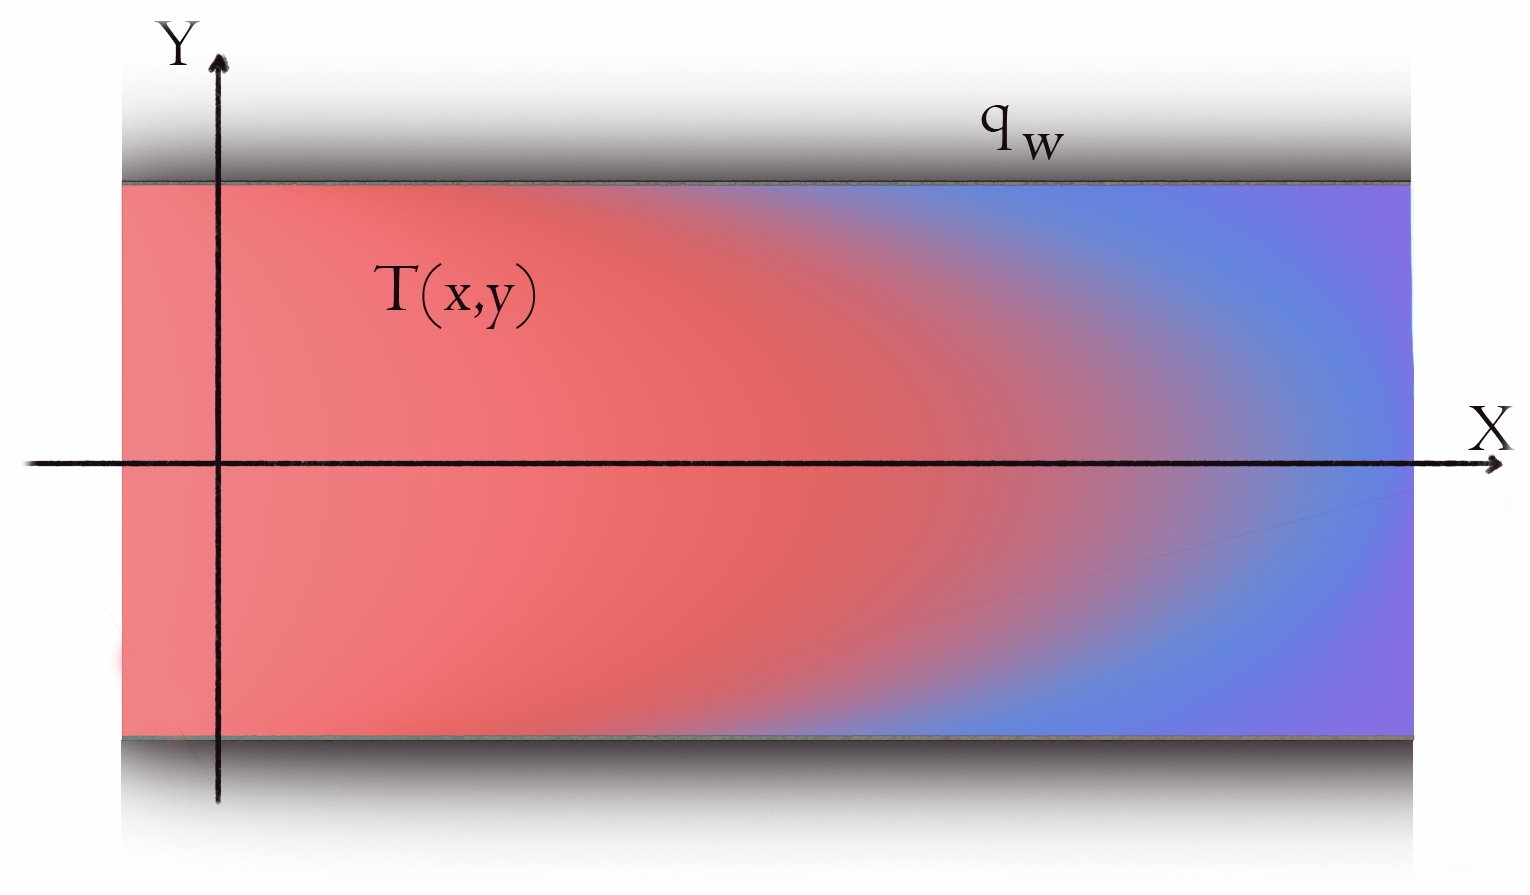
\includegraphics[angle=0, scale=0.14]{imagemtermico}
				\caption{Representação gráfica do domínio térmico do sistema.}
				\label{temperatura}
			\end{figure}
			\end{minipage}
		\end{frame}
		
		
		
		
		
		
		\begin{frame}
		\frametitle{Desenvolvendo a diferença de temperatura na equação}
		\begin{equation}
		\begin{split}
		\frac{\partial ( \overline{T^\ast + T_w}  ) }{\partial t} +
		\frac{\partial{}}{\partial{x}} \left(\overline{(T^\ast + T_w)^\prime u^\prime}\right) + \frac{\partial{}}{\partial{x}}\left(\overline{(T^\ast + T_w)} \ \overline{u}\right)+  \\
		\frac{\partial{}}{\partial{y}} \left(\overline{(T^\ast + T_w)^\prime v^\prime}\right) + \frac{\partial{}}{\partial{y}}\left(\overline{(T^\ast + T_w)} \ \overline{v}\right) = \\
		{\frac{\partial{}}{\partial{x}}} \left(\alpha {\frac{\partial{\overline{(T^\ast + T_w)}}}{\partial{x}}} \right) +
		{\frac{\partial{}}{\partial{y}}} \left(\alpha {\frac{\partial{\overline{(T^\ast + T_w)}}}{\partial{y}}} \right) .
		\end{split}
		\end{equation}
		\begin{center}\begin{equation}\begin{split}
		\frac{\partial ( \overline{ T^\ast + T_w } ) }{\partial t} +
		\frac{\partial{}}{\partial{x}} \left(\overline{T_w^{\prime} u^{\prime}}\right) +\frac{\partial{}}{\partial{x}} \left(\overline{{T^{\ast}}^{\prime} u^{\prime}}\right)
		+\frac{\partial{}}{\partial{x}}\left(\overline{u} \ \overline{T^{\ast}}\right)+ 
		\frac{\partial{}}{\partial{x}}\left(\overline{u} \ \overline{T_w}\right)+ 
		\\
		\frac{\partial{}}{\partial{y}} \left(\overline{{T^{\ast}}^{\prime} v^{\prime}}\right)+
		\frac{\partial{}}{\partial{y}} \left(\overline{T_w^\prime v^\prime}\right) + \frac{\partial{}}{\partial{y}}\left(\overline{v} \ \overline{T^\ast}\right) +
		\frac{\partial{}}{\partial{y}}\left(\overline{v} \ \overline{T_w}\right) 
		= 
		\\
		{\frac{\partial{}}{\partial{x}}} \left(\alpha {\frac{\partial{\overline{(T^\ast + T_w)}}}{\partial{x}}} \right) +
		{\frac{\partial{}}{\partial{y}}} \left(\alpha {\frac{\partial{\overline{(T^\ast + T_w)}}}{\partial{y}}} \right) .
		\end{split}\end{equation}\end{center}
		\end{frame}
		
		
		
		
		
		\begin{frame}
			\frametitle{Simplificações chave na velocidade}
			$\bullet$ Para a velocidade, devem ser feitas as considerações de que é um sistema em regime permanente e unidimensional.
			Assim, na equação da velocidade, teremos as seguintes simplificações:
			\begin{equation}
			\begin{split}
			\color{red}\frac{\partial \overline{u}}{\partial t} \color{black}+\color{red} \frac{\partial \overline{u^2}}{\partial x} \color{black}+\color{red} \frac{\partial \overline{u} \ \color{blue}\overline{v}\color{red}}{\partial y}\color{black} + \color{red} \frac{\partial \overline{u} \ \color{blue}\overline{w}\color{red}}{\partial z} \color{black} =  - \frac{1}{\rho} \frac{\partial \overline{{p}}}{\partial x} + \frac{\partial}{\partial x} \left( \nu \color{red}\frac{\partial \overline{u}}{\partial x} \color{black} - \overline{{u^\prime}^2}\right) + \frac{\partial}{\partial y} \left( \nu \frac{\partial \overline{u}}{\partial y} - \overline{{u^\prime  v^\prime}}\right) \\
			+ \color{red}\frac{\partial}{\partial z} \left( \nu  \frac{\partial \overline{u}}{\partial z} - \overline{ u ^\prime w ^\prime} \right) \color{black}
			\end{split}
			\end{equation}
			\begin{equation}
			\frac{1}{\rho} \frac{\partial \overline{p}}{\partial x} = \frac{\partial}{\partial y} \left( \nu \frac{\partial \overline{u}}{\partial y} - \overline{u^\prime v^\prime}\right)  
			\end{equation}
		\end{frame}
		
		
		
		
		
		\begin{frame}
		\frametitle{Simplificações chave na temperatura}
		$\bullet$ Para a temperatura, foi considerado um regime permanente, derivadas nulas quanto à temperatura e diferença de temperatura, além de que considerou-se a temperatura de parede estável, ou seja, sem flutuações. 
	 	\begin{center}
	 	\begin{equation*}
	 		\begin{split}
	 		\color{red}\frac{\partial ( \overline{ T^\ast + T_w } ) }{\partial t} \color{black} +
	 		\frac{\partial{}}{\partial{x}} \left(\overline{ \color{red}T_w^{\prime} \color{black} u^{\prime}}\right) +
	 		\color{red}\frac{\partial{}}{\partial{x}} \left(\overline{{T^{\ast}}^{\prime} u^{\prime}}\right)+ \color{black}
	 		\color{red} \frac{\partial{}}{\partial{x}}\left(\overline{u} \ \overline{T^{\ast}}\right) \color{black}+ 
	 		\frac{\partial{}}{\partial{x}}\left(\overline{u} \ \overline{T_w}\right)+ 
	 		\\
	 		\frac{\partial{}}{\partial{y}} \left(\overline{{T^{\ast}}^{\prime} v^{\prime}}\right)+
	 		\frac{\partial{}}{\partial{y}} \left(\overline{\color{red}T_w^\prime \color{black} v^\prime}\right) + \frac{\partial{}}{\partial{y}}\left(\color{red}\overline{v} \color{black} \ \overline{T^\ast}\right) +
	 		\frac{\partial{}}{\partial{y}}\left(\color{red}\overline{v}\color{black} \ \overline{T_w}\right) 
	 		= 
	 		\\
	 		\color{red}{\frac{\partial{}}{\partial{x}}} \left(\alpha {\frac{\partial{\overline{(T^\ast + T_w)}}}{\partial{x}}} \right) \color{black}+
	 		{\frac{\partial{}}{\partial{y}}} \left(\alpha {\frac{\partial{\overline{(T^\ast + \color{red} T_w \color{black})}}}{\partial{y}}} \right) .
	 		\end{split}
	 	\end{equation*}
 		\end{center}
 		\begin{equation}\label{equation_var}
 			{\frac{\partial{}}{\partial{y}}} \left(\alpha {\frac{\partial{\overline{T^\ast}}}{\partial{y}}}   
 			- \left(\overline{ T^{\ast\prime} v^\prime}\right) \right)
 			= 
 			\overline{u}\frac{\partial{}}{\partial{x}}\left(\overline{T_w}\right)  .
 		\end{equation}
		\end{frame}
	
		
		
		
		
		
		\begin{frame}
			\frametitle{Hipótese de Boussinesq}
			$\bullet$ Dessa forma fica o fluxo turbulento para se modelar. O termo $\overline{T^{\ast\prime}  v^\prime}$ pode ser desenvolvido segundo a hipótese de Boussinesq, que postula:
			\begin{equation}\label{bou}
			-\left(\overline{ u^\prime  v^\prime}\right) = 
			\nu_t \frac{\partial{\overline{u}}}{\partial{y}}
			\implies
			-\left(\overline{ T^{\ast\prime}  v^\prime}\right) = 
			\alpha_t \frac{\partial{\overline{T^\ast}}}{\partial{y}}.
			\end{equation}
			Assim, desenvolvendo a equação: 
			\\
				\begin{equation}
				{\frac{\partial{}}{\partial{y}}} \left(\alpha {\frac{\partial{\overline{T^\ast}}}{\partial{y}}}   
				+ \alpha_t  \frac{\partial \overline{T^\ast}}{\partial y} \right)
				= 
				\overline{u}\frac{\partial{}}{\partial{x}}\left(\overline{T_w}\right) . 
				\end{equation}
		\end{frame}
	
	
	
	
		
		\begin{frame}
			\frametitle{Comprimento de mistura de Prandtl}
			$\bullet$ Dessa forma, surge o termo da difusidade térmica turbulenta $\alpha_t$ que precisa ser modelado. Uma nova variável deve ser introduzida, o número de Prandtl turbulento, como segue:
			\begin{equation}
				Pr_t = \frac{\nu_t}{\alpha_t}.
			\end{equation} 
			Assim, temos o valor do $\nu_t$ que precisa ser modelado. O valor do número de Prandtl turbulento de $ Pr_t = 0.71$ tem sido utilizado na literatura.
			Com o modelo do comprimento de mistura de Prandtl, postula-se que:
			\begin{equation}
			\nu_t = {l_m}^2 \left| \frac{\partial \overline{u}}{\partial y} \right|.
			\end{equation}
		\end{frame}
		
		
		
		
		
		\begin{frame}
			\frametitle{Substituindo o comprimento de mistura na equação principal}	
			$\bullet$ O comprimento de mistura introduz um módulo no modelo diferencial e o parâmetro do número de Prandtl turbulento.   
			\\
				\begin{equation}
				{\frac{\partial{}}{\partial{y}}} \left( \left( \alpha   
				+ \frac{\nu_t}{Pr_t} \right) \frac{\partial \overline{T^\ast}}{\partial y} \right)
				= 
				\overline{u}\frac{\partial{}}{\partial{x}}\left(\overline{T_w}\right)  .
				\end{equation}
			\begin{equation}
			{\frac{\partial{}}{\partial{y}}} \left( \left( \alpha   
			+ \frac{{l_m}^2 \left| \frac{\partial \overline{u}}{\partial y} \right|}{Pr_t} \right) \frac{\partial \overline{T^\ast}}{\partial y} \right)
			= 
			\overline{u}\frac{\partial{}}{\partial{x}}\left(\overline{T_w}\right)  .
			\end{equation}
		\\
		É possível notar, ao se analisar o domínio dinâmico, que para valores positivos de $ y $, a primeira derivada da velocidade sempre será negativa, visto que pelos princípios de Dirichlet e Neumman, tem-se uma velocidade que diminui com o aumento de $ y $. Assim, temos:\\
			\begin{equation}
			{\frac{\partial{}}{\partial{y}}} \left( \left( \alpha   
			- \frac{{l_m}^2}{Pr_t}\frac{\partial \overline{u}}{\partial y} \right) \frac{\partial \overline{T^\ast}}{\partial y} \right)
			= 
			\overline{u}\frac{\partial{}}{\partial{x}}\left(\overline{T_w}\right)  .
			\end{equation}
		\end{frame}	
	
	
	
	
		\begin{frame}
			\frametitle{Um modelo para o comprimento de mistura de Prandtl}
			Um modelo para $l_m$ deve ser estabelecido. Para tal, se observou os estudos experimentais de Nikuradse, com o qual modelou-se esse parâmetro como segue.
			\begin{equation}
			L\left(\frac{y}{R}\right) = \frac{l_m}{R} = 0.14 - 0.08 \left(\frac{y}{R}\right)^2 - 0.06\left(\frac{y}{R}\right)^4.
			\end{equation}
			Para enriquecer ainda mais o modelo, Cebeci e Bradshaw acrescentaram a função de amortecimento de Van Driest:
			\begin{equation}
			L\left(\frac{y}{R}\right)  = \frac{l_m}{R} = \left(\frac{l_m}{R} = 0.14 - 0.08 \left(\frac{y}{R}\right)^2 - 0.06\left(\frac{y}{R}\right)^4\right)\left\{  1 - e^{[(\tilde{y} - 1) \frac{Re_\tau}{26}]}\right\}.
			\end{equation}
			Assim, tem-se o comprimento de mistura definido por:
			\begin{equation}
			lm = L R.
			\end{equation}
			Sendo $ L $ uma função em $ y $. É importante notar que neste momento foi introduzida a constante de Cebeci, que é o número $ 26 $ que divide o $ Re_\tau $.
		\end{frame}
		
		
		
		
		
		\begin{frame}
			\frametitle{Substituindo o comprimento de mistura nas equações}
			$\bullet$ É importante observar que a função $ L(\frac{y}{R}) $ já está Adimensionalizada.
				\begin{equation}
				{\frac{\partial{}}{\partial{y}}} \left( \left( \alpha   
				- \frac{{L}^2 R ^2}{Pr_t}\frac{\partial \overline{u}}{\partial y} \right) \frac{\partial \overline{T^\ast}}{\partial y} \right)
				= 
				\overline{u}\frac{\partial{}\left(\overline{T_w}\right)  }{\partial{x}}.
				\end{equation}
		\end{frame}
		
		
		
		
		
		\begin{frame}
			\frametitle{Desenvolvendo a equação dinâmica}
			$\bullet$ Desenvolvendo a equação dinâmica foi possível se explicitar de forma exata a primeira derivada da velocidade.
			\begin{equation}
			\int \frac{1}{\rho} \frac{\partial \overline{p}}{\partial x} dy = \int \frac{\partial}{\partial y} \left( \nu  \frac{\partial \overline{u}}{\partial y} - {L}^2 R ^2 \left(\frac{\partial \overline{u}}{\partial y}\right) ^ 2 \right) dy  
			\end{equation}
			\begin{equation}
			\frac{1}{\rho} \frac{\partial \overline{p}}{\partial x} \int 1 dy = \int \frac{\partial}{\partial y} \left( \nu  \frac{\partial \overline{u}}{\partial y} - {L}^2 R ^2 \left(\frac{\partial \overline{u}}{\partial y}\right) ^ 2 \right) dy  
			\end{equation}
			\begin{equation}
			y \frac{1}{\rho} \frac{\partial \overline{p}}{\partial x} =  \nu  \frac{\partial \overline{u}}{\partial y} - {L}^2 R ^2 \left(\frac{\partial \overline{u}}{\partial y}\right) ^ 2 
			\end{equation}
			\begin{equation}
			{L}^2 R ^2 \left(\frac{\partial \overline{u}}{\partial y}\right) ^ 2 - \nu  \frac{\partial \overline{u}}{\partial y} + y \frac{1}{\rho} \frac{\partial \overline{p}}{\partial x} = 0
			\end{equation}
			Observando-se a conformação em forma de polinômio de segundo grau, retirou-se as raízes, onde só uma delas teve consistência física.
			\begin{equation}
			\frac{\partial \overline{u}}{\partial y} = \frac{2 y \frac{1}{\rho}\frac{\partial \overline{p}}{\partial x} }{ \nu + \sqrt{\nu ^2 + 4 y \frac{1}{\rho} \frac{\partial \overline{p}}{\partial x} L ^2 R ^2}}
			\end{equation}
		\end{frame}
			
		
		
		
		\begin{frame}
		\frametitle{Modelo referente ao gradiente de pressão}
		$\bullet$ Para este desenvolvimento se utilizou a definição da tenção cisalhante e uma análise segundo a primeira lei de Newton.
		\begin{equation}
		u_\tau = \sqrt{\frac{\left| \tau_w \right|}{\rho}}
		\end{equation}
		\begin{equation}
		p_1 2R = 2 \tau_w \Delta x + p_2 2 R
		\end{equation}
		Assim, desenvolvendo e substituindo, temos:
		\begin{equation}
		\frac{\tau_w}{R} = \frac{(p_1 - p_2)}{\Delta x}
		\end{equation}
		\begin{equation}
		- \frac{\partial \overline{p}}{\partial x} = \frac{\tau_w}{R} = \frac{u_\tau^2 \rho}{R} 
		\end{equation}
		\end{frame}
	
	
	
	
	
	
		\begin{frame}
			\frametitle{Adimensionalização}
			$\bullet$ Para se comparar mais facilmente os modelos à literatura, adimensionalizou-se as equações segundo coordenadas de parede. Foi considerado: $ \tilde{y} = \frac{y . Re_\tau}{R} $, $ \tilde{\overline{u}} = \frac{\overline{u}}{u_\tau} $ , $ \tilde{\overline{T}} = \frac{\overline{T}}{T_\tau} $ , $Re_\tau = \frac{u_\tau R}{\nu}$, $Pr_t = \frac{\nu_t}{\alpha_t}$, $Pr = \frac{\nu}{\alpha}$ e $T_\tau = \frac{q_w}{\rho C_p u_\tau}$, $\frac{\partial{\left(T_m\right)}}{\partial{x}} = \frac{q_w}{u_m  R \rho  C_p } $, $\frac{\partial \overline{p}}{\partial x} = - \frac{u_\tau^2 \rho}{R} $.
			\\
				\begin{equation}
				{\frac{\partial{}}{\partial{y}}} \left( \left( \alpha   
				- \frac{{L}^2 R ^2}{Pr_t}\frac{\partial \overline{u}}{\partial y} \right) \frac{\partial \overline{T^\ast}}{\partial y} \right)
				= 
				\overline{u}\frac{\partial{}\left(\overline{T_w}\right)  }{\partial{x}}.
				\end{equation}
				\begin{equation}
				{\frac{\partial{}}{\partial{\tilde{y}}}} \left( \left( \frac{Re_\tau}{Pr}   
				- \frac{{L}^2 Re_\tau ^3}{Pr_t}\frac{\partial \tilde{\overline{u}}}{\partial \tilde{y}} \right) \frac{\partial \tilde{\overline{T^\ast}}}{\partial \tilde{y}} \right)
				= 
				\frac{\tilde{\overline{u}}}{\tilde{u_m}}.
				\end{equation}
		\end{frame}
	
	
	
		\begin{frame}
			\frametitle{O desenvolvimento dinâmico}
			$\bullet$ É importante notar como há a velocidade na equação principal, ou seja, para o desenvolvimento do domínio térmico fez-se necessário o desenvolvimento do perfil dinâmico do canal. Para isso utilizou-se uma metodologia RANS previamente estabelecida, como segue: 
				\begin{equation}
				\frac{\partial \tilde{\overline{u}}}{\partial \tilde{y}} = - \frac{2 \tilde{y} \frac{1}{Re_\tau} }{ 1 + \sqrt{ 1 + 4 L ^2 Re_\tau ^2 \tilde{y}}}.
				\end{equation}	
				
			Dessa forma, tem-se a primeira derivada da velocidade de forma exata.
		\end{frame}
	
	

	
	
	\section{Modelo numérico}
		
	
	
	
		
		\begin{frame}
			\frametitle{Discretização do espaço}
			\begin{minipage}[h!]{0.5\textwidth}
			$\bullet$ Para discretizar o espaço, foi formulado um domínio Euleriano. Para a velocidade foi aplicado um Runge-kutta de quarta ordem, enquanto a temperatura foi arranjada em um sistema de diferenças centradas que teve de ser resolvido implicitamente. O domínio dinâmico foi resolvido primeiro, e seu resultado numérico fora utilizado no desenvolvimento do perfil térmico. Quanto à localização das células, foi determinado um centro de célula na parede, e um ponto entre células no centro do canal, sendo o restante das unidades de espaço distribuídas uniformemente para todo o canal.
			\end{minipage}\hfill
			\begin{minipage}[h!]{0.45\textwidth}
			\begin{figure}
				\centering
				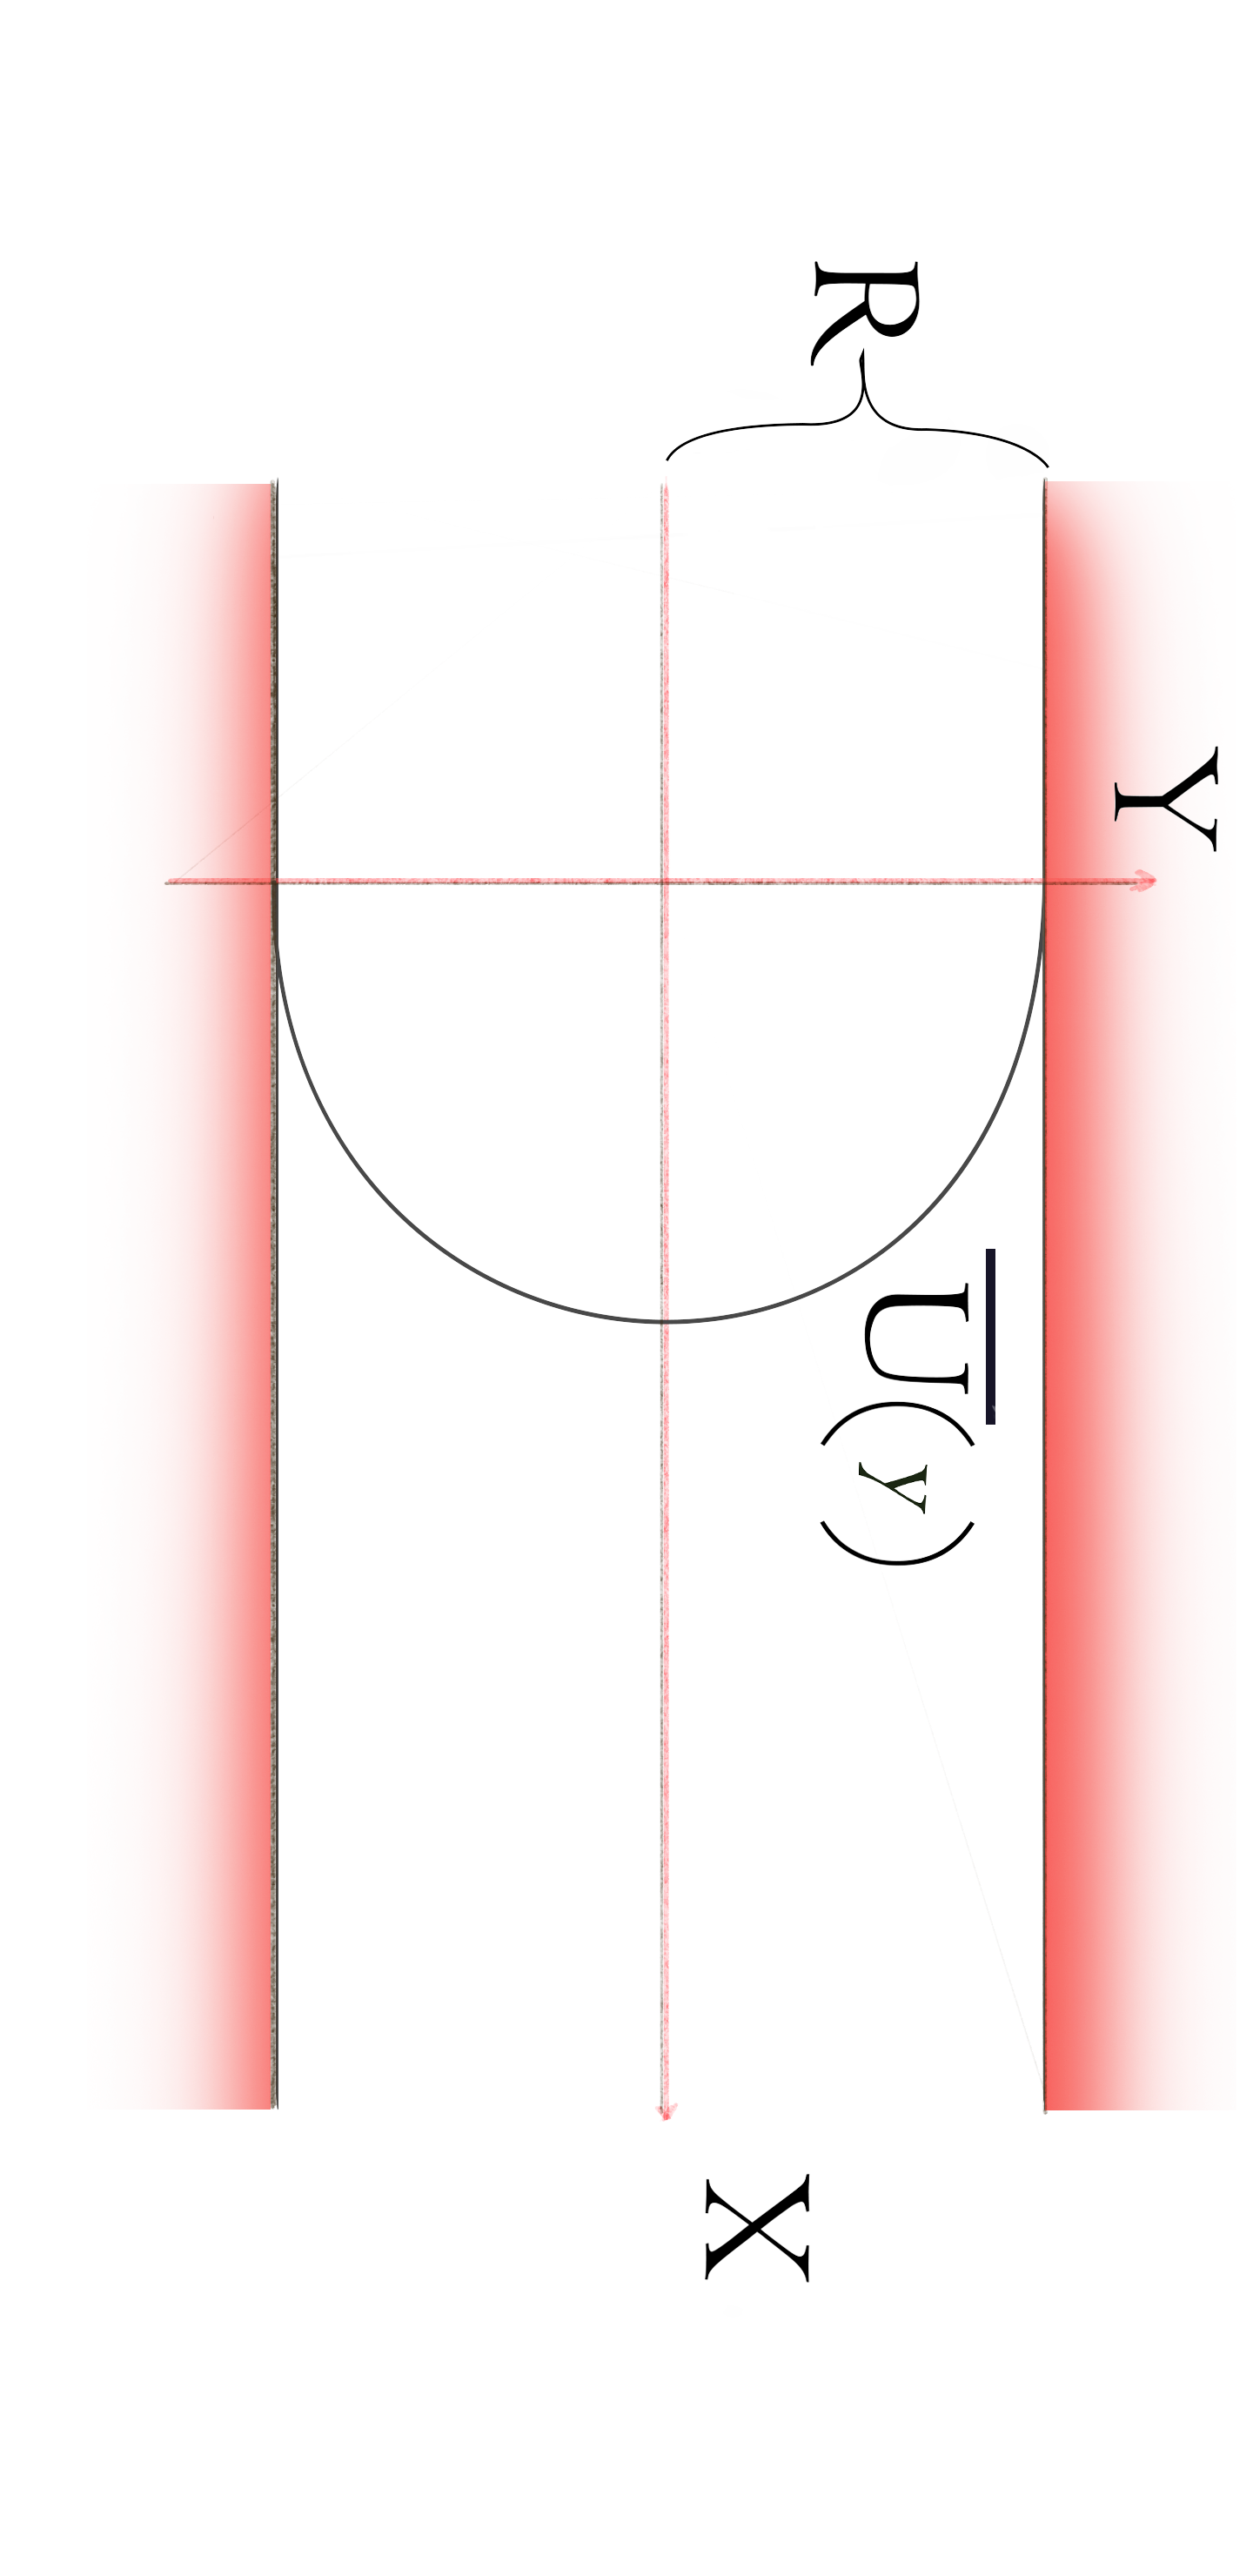
\includegraphics[angle=90, scale=0.06]{canalvermelho}
				\caption{Representação gráfica do domínio do sistema.}
				\label{sistema}
			\end{figure}
			\end{minipage}\\
		\end{frame}
	
	
	
	
	
			\begin{frame}
		\begin{figure}
			\centering
			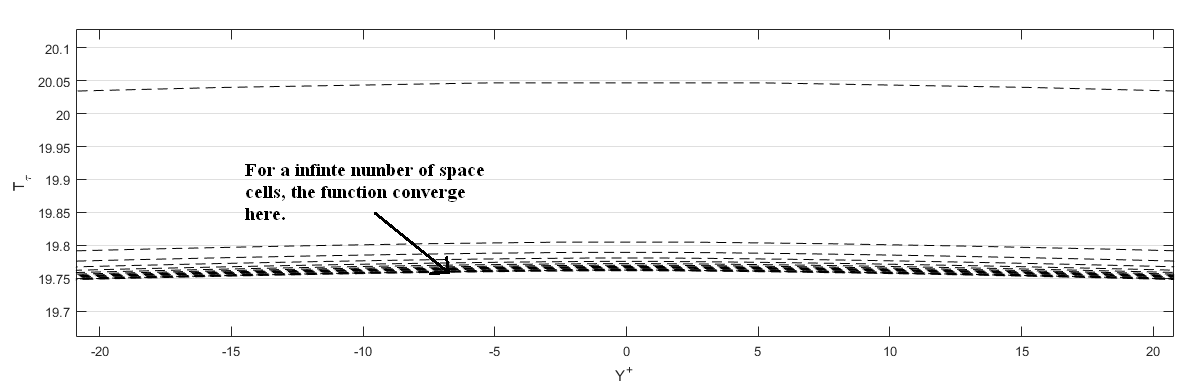
\includegraphics[angle=0, scale=0.42]{convergnciaprimeira}
			\caption{Convergência e independência de malha.}
			\label{convergencia}
		\end{figure}
	\end{frame}
		
	
	
	
		
	\section{Resultados}
		\begin{frame}
			\frametitle{Simulações preliminares: $Pr_t= 0.71$ , $A = 26 $}
				$\bullet$ Inicialmente utilizou-se o Prandtl turbulento como um valor da literatura, de 0.71, onde se obteve os seguintes resultados:\\
			\begin{minipage}[h!]{0.45\textwidth}
			\begin{figure}
				\centering
				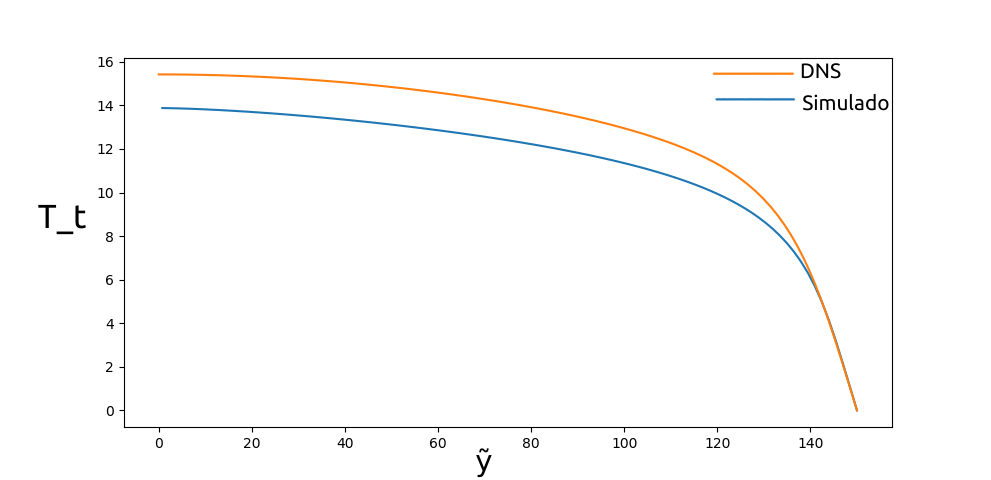
\includegraphics[angle=0, scale=0.28]{150orto}
				\caption{Resultado para $Re_\tau = 150$. L2 = 1.36 }
			\end{figure}
			\end{minipage}\hfill
				\begin{minipage}[h!]{0.45\textwidth}
				\begin{figure}
					\centering
					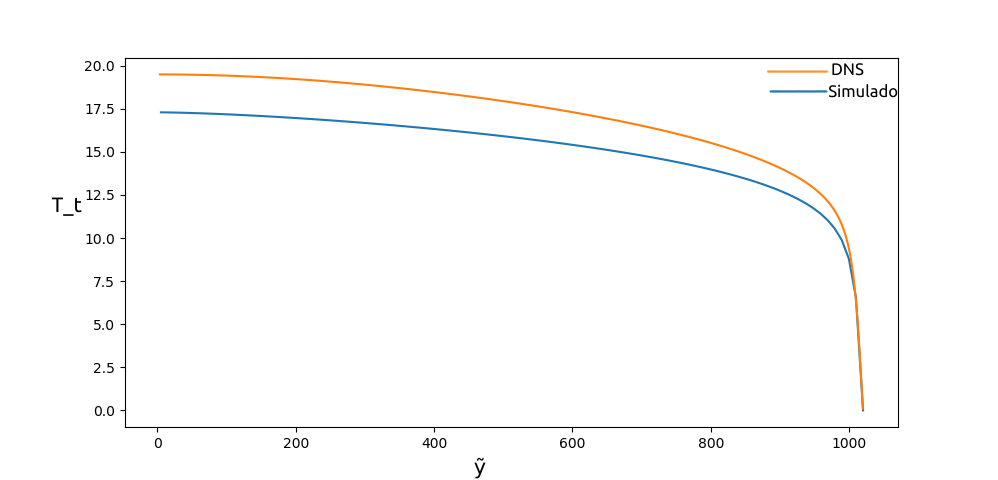
\includegraphics[angle=0, scale=0.28]{1020orto}
					\caption{Resultado para $Re_\tau = 1020$. L2 = 1.77}
				\end{figure}
			\end{minipage}		
		\end{frame}
	
	
	
	
		
		\begin{frame}
		\frametitle{Estudo do número de Prandtl turbulento fornecido por DNS}
		\begin{minipage}[h!]{0.45\textwidth}
			$\bullet$ Observou-se o resultado para quando o número de Prandtl turbulento do DNS era utilizado, obtendo-se uma norma L2 de $0.19$ para $Re_t = 640$. Assim se identificou que o problema estava na parametrização do Prandtl turbulento que passou a ser o foco da pesquisa. 
		\end{minipage}\hfill
		\begin{minipage}[h!]{0.45\textwidth}
			\begin{figure}
				\centering
				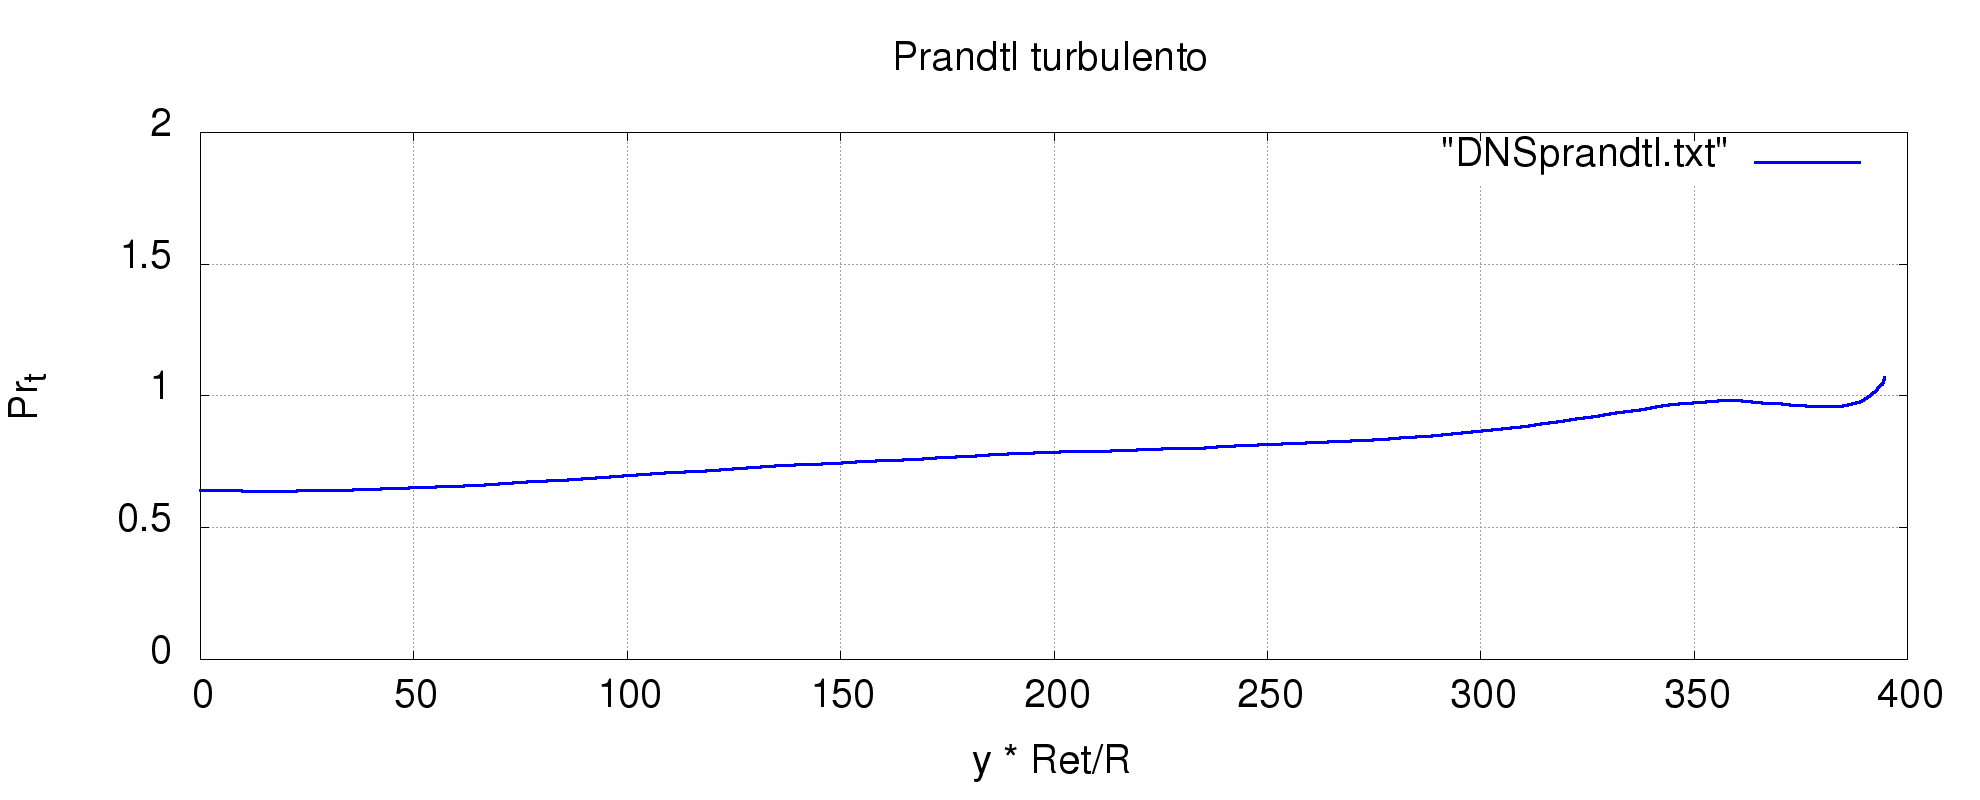
\includegraphics[angle=0, scale=0.12]{perfisPrandtlturb_Ret_Pt}
				\caption{Vetor com o número de Prandtl turbulento em função da coordenada $ y $ no canal.}
			\end{figure}
		\end{minipage}	\\
		Assim iniciou-se o esforço de se propor uma parametrização ajustada para o número de Prandtl turbulento.
		Nesse sentido procurou-se ajustar um valor para o qual o erro fosse mínimo quando feita a comparação da simulação com DNS.
		\end{frame}
	
	
		\begin{frame}
		\frametitle{Ajustando um valor de Prandtl turbulento}
		\begin{minipage}[h!]{0.45\textwidth}
			$\bullet$ Escreveu-se um algoritmo que buscava um erro mínimo para a função, considerando o número de Prandtl turbulento como uma variável editável e o erro menor como o padrão de interesse. 
			
			Obteve-se um número de Prandtl turbulento ajustado de $ 0.905 $ Para o número de Reynolds turbulento de $1020$.
			
			Tal valor foi aplicado a todo o domínio.
		\end{minipage}
			\begin{minipage}[h!]{0.2\textwidth}
			\end{minipage}
			\begin{minipage}[h!]{0.45\textwidth}
			\begin{figure}
				\centering
				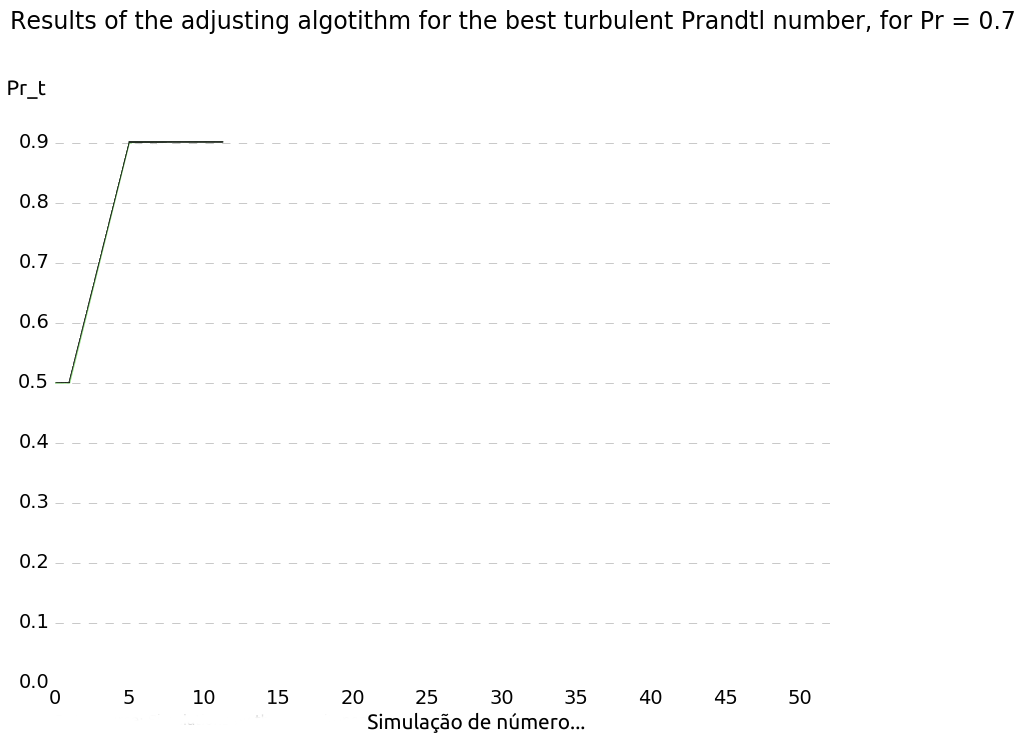
\includegraphics[angle=0, scale=0.32]{oloco}
				\caption{Resultado para $Re_\tau = 1020$. L2 = 0.151}
			\end{figure}
		\end{minipage}	
		\end{frame}
		
		
		
		
		
		\begin{frame}
		\frametitle{Ajuste de um valor fixo ideal: $Pr_t = 0.905$ , $A = 26$}
		$\bullet$Simulações com o número de Prandtl turbulento ajustado fixo em $Re_\tau = 1020$:  \\
		\begin{minipage}[h!]{0.45\textwidth}
			 \begin{figure}
			 	\centering
			 	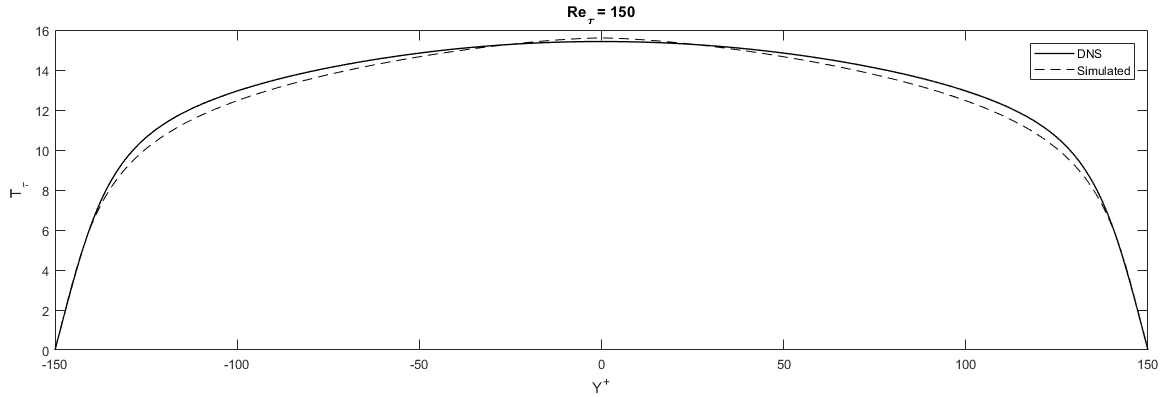
\includegraphics[angle=0, scale=0.22]{150segundo}
			 	\caption{Resultado para $Re_\tau = 150$. L2 = 0.341}
			 \end{figure}
			 \begin{figure}
			 	\centering
			 	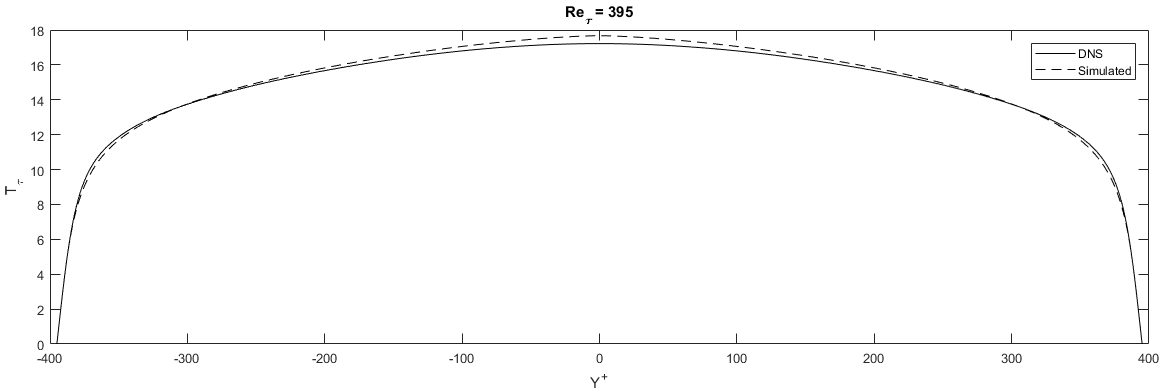
\includegraphics[angle=0, scale=0.22]{395segundo}
			 	\caption{Resultado para $Re_\tau = 395$. L2 = 0.23}
			 \end{figure}
		\end{minipage}\hfill
		\begin{minipage}[h!]{0.45\textwidth}
			\begin{figure}
				\centering
				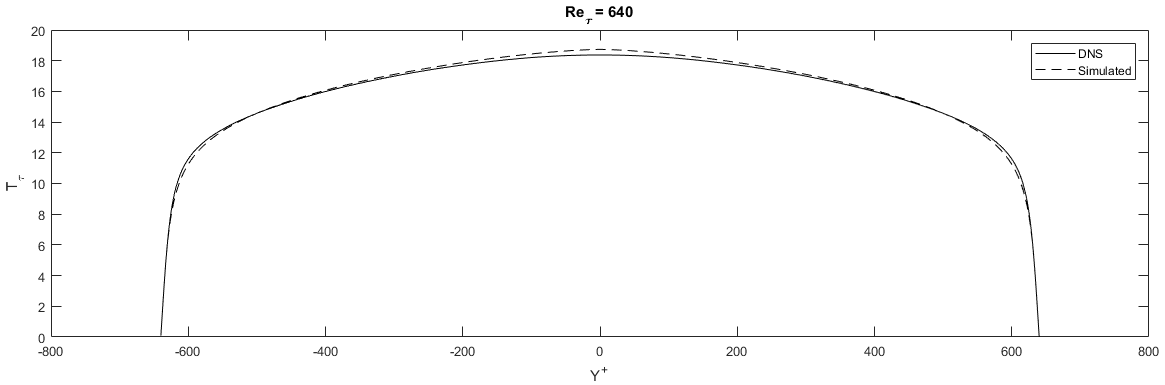
\includegraphics[angle=0, scale=0.22]{640segundo}
				\caption{Resultado para $Re_\tau = 640$. L2 = 0.192}
			\end{figure}
			\begin{figure}
				\centering
				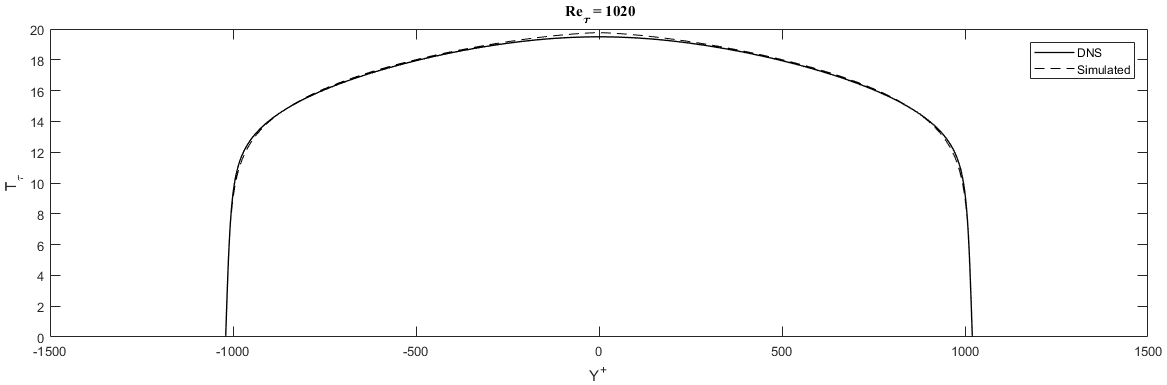
\includegraphics[angle=0, scale=0.22]{1020segundo}
				\caption{Resultado para $Re_\tau = 1020$. L2 = 0.151}
			\end{figure}
		\end{minipage}		
		\end{frame}	
	
	
	
	
		
		\begin{frame}
		\frametitle{Algoritmo de otimização}
		$\bullet$ Para se obter uma curva que contemplasse os números de Reynolds em todo o domínio, se desenvolveu-se um algoritmo que otimizava a um Prandtl turbulento ideal para cada número de Reynolds turbulento disponível em DNS.\\
		\begin{minipage}[h!]{0.45\textwidth}
			\begin{figure}
				\centering
				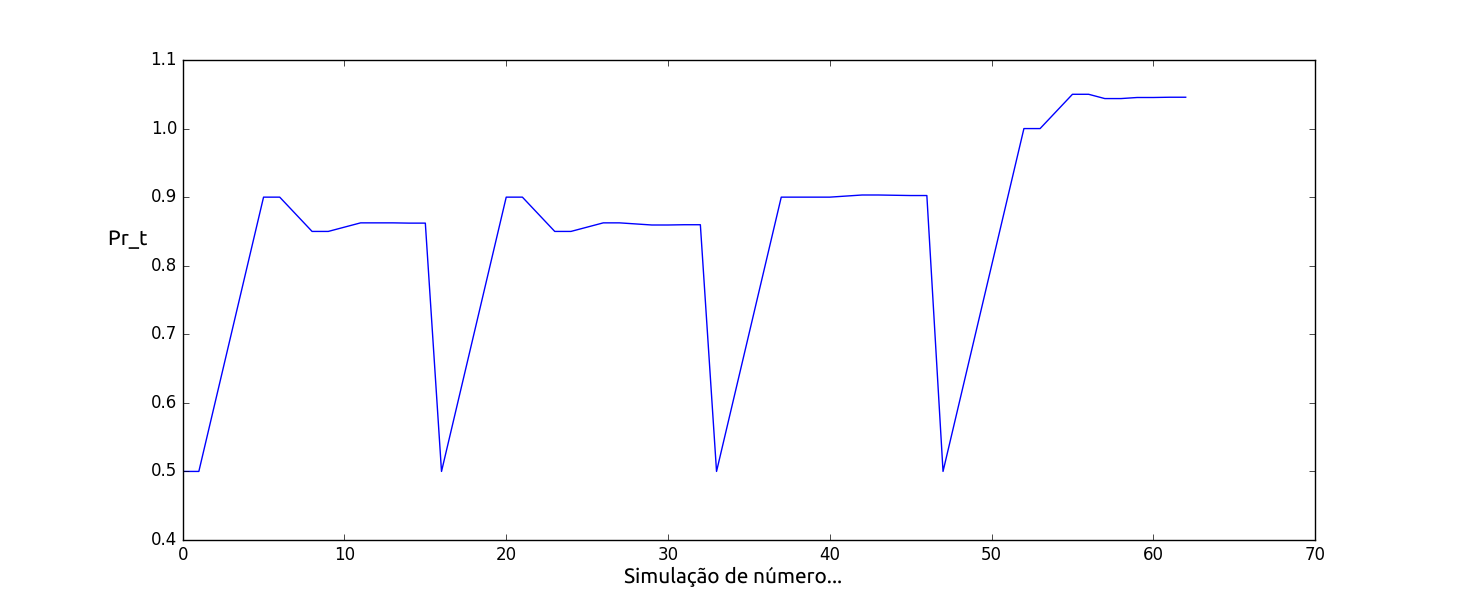
\includegraphics[angle=0, scale=0.22]{convergnciacima}
				\caption{Algoritmo para valores ótimos. Com início abaixo do valor estimado.}
			\end{figure}
		\end{minipage}\hfill
		\begin{minipage}[h!]{0.45\textwidth}
			\begin{figure}
				\centering
				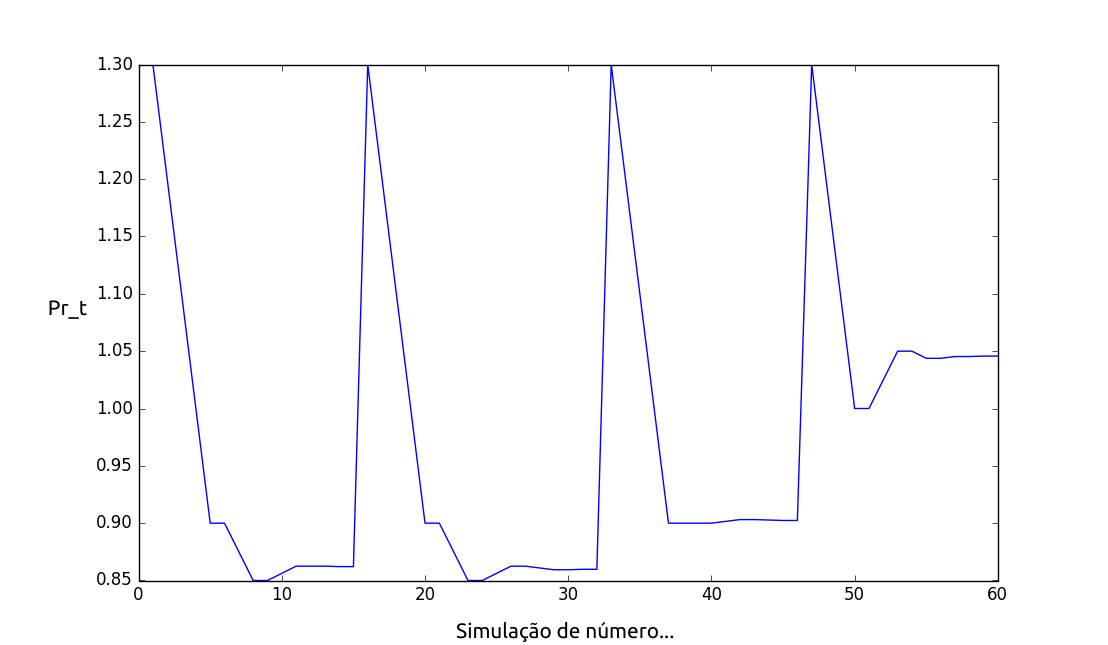
\includegraphics[angle=0, scale=0.22]{convergnciabaixo}
				\caption{Algoritmo para valores ótimos. Com início acima do valor estimado.}
			\end{figure}
		\end{minipage}\\
		Como forma de se ter certeza de ter se chegado a um mínimo global, executou-se o algorítimo a partir de um ponto acima e de um ponto abaixo do inferido. 		
		\end{frame}	
	
	
	
	
		\begin{frame}
		\frametitle{Ajuste dos valores obtidos}
		\begin{minipage}[h!]{0.45\textwidth}
			$\bullet$ Executando um ajuste de curva polinomial, obteve-se a seguinte relação:
			\begin{equation}
			\begin{split}
			Pr_t = 1,3 * 10^{-11} Re_\tau^3 - 7,1 * 10^{-8} Re_\tau^2 \\ + 0,0001 Re_\tau + 0,87 
			\end{split}
			\end{equation}
			Assim, desenvolveu-se um modelo ajustado para o número de Prandtl turbulento em função do número de Reynolds turbulento.
		\end{minipage}\hfill
		\begin{minipage}[h!]{0.45\textwidth}
			\begin{figure}
				\centering
				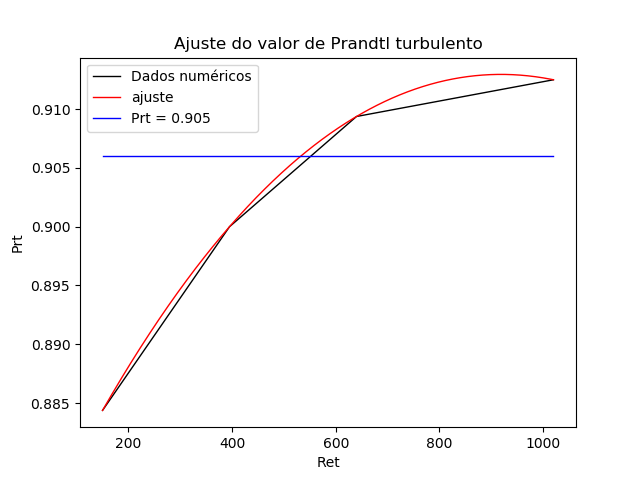
\includegraphics[angle=0, scale=0.41]{ajustePrandtl}
				\caption{Ajuste de um modelo para $Pr_t$ variável.}
			\end{figure}
		\end{minipage}\\
		\end{frame}	
		
		
		
	
	
		\begin{frame}
		\frametitle{Ajuste do valor de Cebeci}
		\begin{minipage}[h!]{0.45\textwidth}
			$\bullet$ A partir dos pontos resultantes do algoritmo de otimização, se desenvolveu o modelo ajustado para o valor de Cebeci. Como segue:
			\begin{equation}
			A = \frac{Re_\tau ^{0.0451 * \ln(Re_\tau)} *e ^ {5.2753} }{Re_\tau ^{0.6094}}
			\end{equation}
		\end{minipage}\hfill
		\begin{minipage}[h!]{0.45\textwidth}
		\begin{figure}
			\centering
			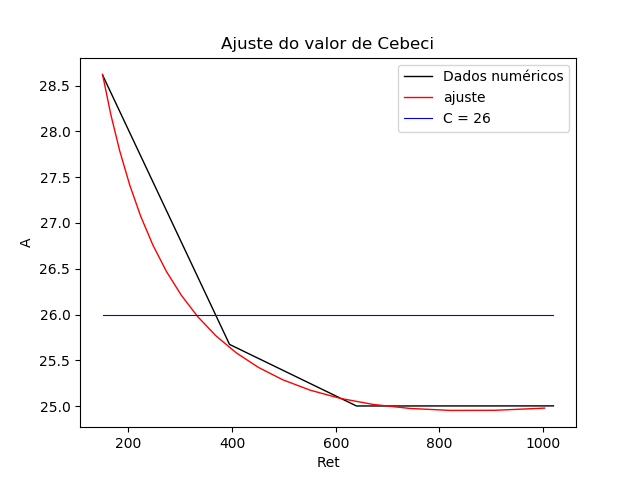
\includegraphics[angle=0, scale=0.42]{ajustecebeci}
			\caption{Ajuste de um modelo para um número de Cebeci variável.}
		\end{figure}
		\end{minipage}
		\end{frame}	

	
	
	
	
		\begin{frame}
		\frametitle{Análise quanto à influencia do número de Prandtl}
		\begin{minipage}[h!]{0.45\textwidth}
		$\bullet$ Estudou-se a influencia do número de Prandtl molecular e observou-se que ele também era uma variável com influencias no erro do método, assim iniciou-se um estudo com o objetivo de se adicionar a influência do valor do número de Prandtl à parametrização do número de Prandtl turbulento. Para isso propôs-se o seguinte modelo:
		\end{minipage}\hfill
		\begin{minipage}[h!]{0.45\textwidth}
		\begin{figure}
			\centering
			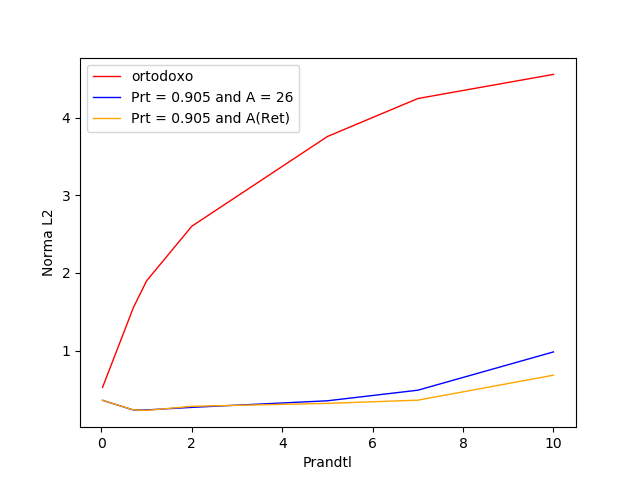
\includegraphics[angle=0, scale=0.38]{analisepr}
			\caption{Observação quanto à influência do número de Prandtl.}
		\end{figure}
		\end{minipage}\\
		\begin{equation}
	\begin{split}
	Pr_t = \left( 1,3 * 10^{-11} Re_\tau^3 - 7,1 * 10^{-8} Re_\tau^2 + 0,0001 Re_\tau + 0,87 \right) \left(  \frac{Pr}{0,71}\right) ^{v}
	\end{split}
	\end{equation}
		\end{frame}
	
	
	
	
			\begin{frame}
	\frametitle{Algoritmo genético de otimização}
	$\bullet$ No ajuste do expoente na expansão da parametrização do número de Prandtl turbulento, utilizou-se um algoritmo evolutivo, que a partir de uma população inicial de casos convergiu para o valor mínimo.\\ 
	\begin{minipage}[h!]{0.24\textwidth}
		\begin{figure}
			\centering
			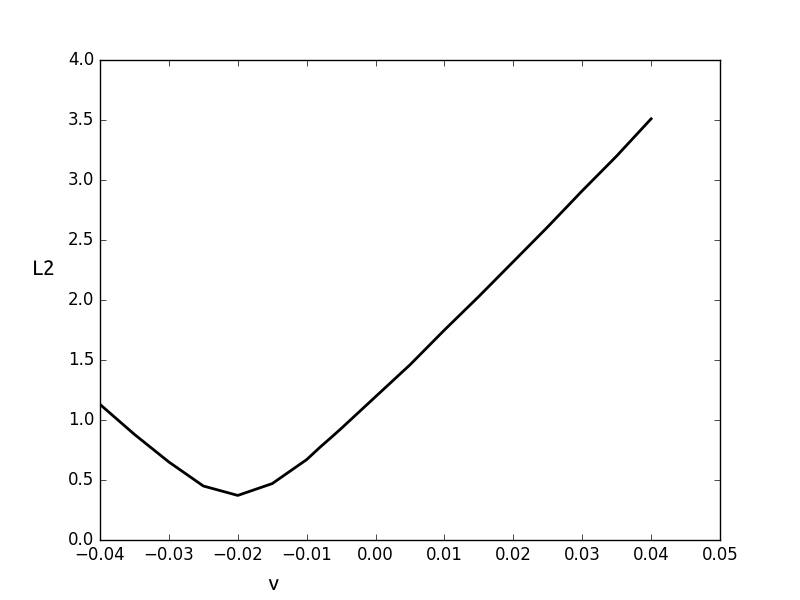
\includegraphics[angle=0, scale=0.20]{A100}
			\caption{Algoritmo para valores ótimos, com malha de 100 unidades.}
		\end{figure}
	\end{minipage}\hfill
	\begin{minipage}[h!]{0.24\textwidth}
		\begin{figure}
			\centering
			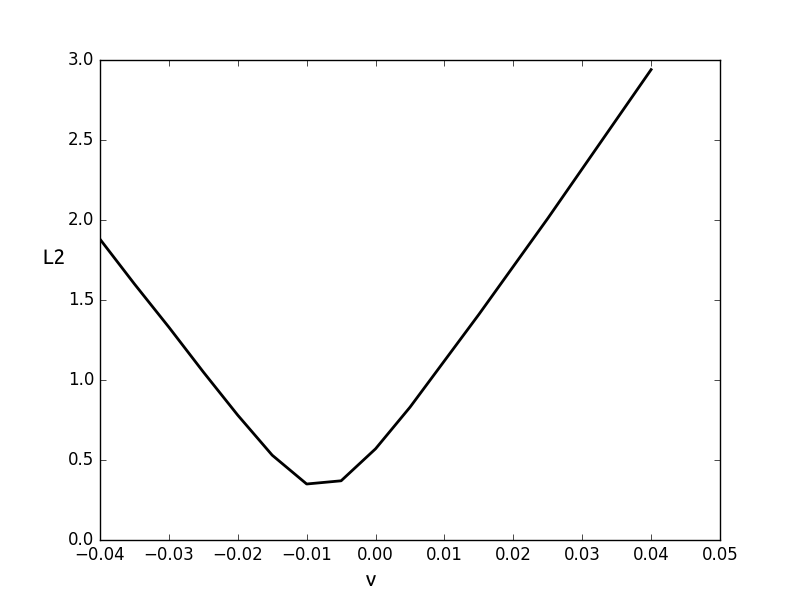
\includegraphics[angle=0, scale=0.20]{A400}
			\caption{Algoritmo para valores ótimos, com malha de 400 unidades.}
		\end{figure}
	\end{minipage}\hfill
\begin{minipage}[h!]{0.24\textwidth}
	\begin{figure}
		\centering
		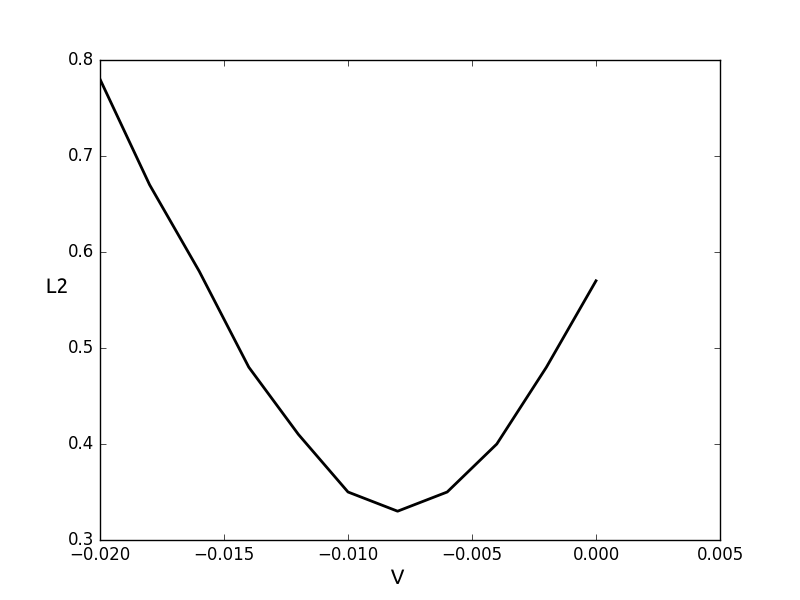
\includegraphics[angle=0, scale=0.20]{A400zoon}
		\caption{Algoritmo para valores ótimos, com malha de 400 unidades, segunda geração.}
	\end{figure}
\end{minipage}	
	\begin{equation}
\begin{split}
Pr_t = \left( 1,3 * 10^{-11} Re_\tau^3 - 7,1 * 10^{-8} Re_\tau^2 + 0,0001 Re_\tau + 0,87 \right) \left(  \frac{Pr}{0,71}\right) ^{-0.008}
\end{split}
\end{equation}	
\end{frame}	
	
	
	
	
	
	
	
		\begin{frame}
		\frametitle{Resultados gerais}
		\begin{minipage}[h!]{0.45\textwidth}
		\animategraphics[trim = {1.7cm 2cm 0 1cm} , scale=2 , loop,controls = true,width=\linewidth]{10}{plot/plot_}{001}{180}
		\end{minipage}\hfill
		\end{frame}
	
	
	
	
	
		\begin{frame}
		\frametitle{Comparação entre os métodos}
		$\bullet$ Seguem alguns recortes do gráfico anterior, explicitando os erros obtidos para um Ret fixo de 395, e um Pr fixo de 0.71.\\
		\begin{minipage}[h!]{0.47\textwidth}
			\begin{figure}
	\centering
	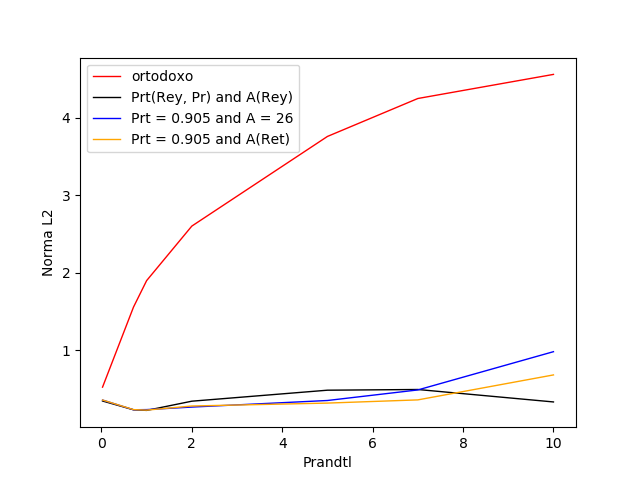
\includegraphics[angle=0, scale=0.39]{finaispr}
	\caption{Resultados gerais para $Re_\tau = 395$}
\end{figure}
		\end{minipage}
		\begin{minipage}[h!]{0.47\textwidth}
		\begin{figure}
			\centering
			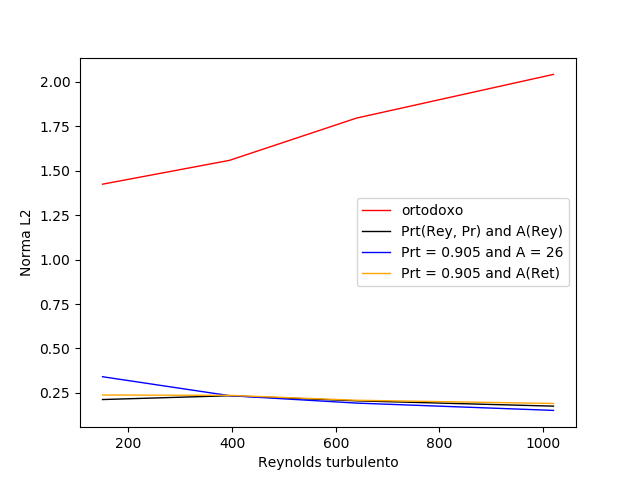
\includegraphics[angle=0, scale=0.39]{finaisRey}
			\caption{Resultados gerais para $Pr = 0.71$}
		\end{figure}
		\end{minipage}\\
		\end{frame}
		
	
	
	
	
	
	
	\section{Agradecimentos}
		
		
		
		
		
			\begin{frame}
				\placelogomflab 
				\frametitle{Agradecimentos}
				\begin{figure}
					\begin{center}
						\begin{tabular}{c c}
							{
\includegraphics[trim=0.0cm 0.0cm 0.0cm 0.0cm,clip=true,height=0.2\textheight]{figuras/petrobras.png}}&{
\includegraphics[trim=0.0cm 0.0cm 0.0cm 0.0cm,clip=true,height=0.2\textheight]{figuras/logo_mflab.png}}\\
							{
\includegraphics[trim=0.0cm 0.0cm 0.0cm 0.0cm,clip=true,height=0.2\textheight]{figuras/cnpq.png}}&{
\includegraphics[trim=0.0cm 0.0cm 0.0cm 0.0cm,clip=true,height=0.2\textheight]{figuras/CAPES.png}}\\
							{
\includegraphics[trim=0.0cm 0.0cm 0.0cm 0.0cm,clip=true,height=0.2\textheight]{figuras/FAPEMIG.jpg}}&{
\includegraphics[trim=0.0cm 0.0cm 0.0cm 0.0cm,clip=true,height=0.2\textheight]{figuras/UFU_black.jpg}}\\
						\end{tabular}
					\end{center}
				\end{figure}
			\end{frame}
			
			
			
			
			
			\begin{frame}
				\placelogomflab 
				\frametitle{Agradecimentos}
				\fontsize{44pt}{7.2}\selectfont
				\begin{center}
					Obrigado.
				\end{center}
			\end{frame}
		
		
		
		
\end{document}




		



%%%%%%%%%%%%%%%%%%%%%%%%%%%%%%%%%%%%%%% Exemplo de formatação de imagens		
%		\begin{frame}
%			\frametitle{Adição de fronteiras extras}
%			\begin{tabular}{c c}
%				
%				{\includegraphics[trim=0.0cm 0.0cm 0.0cm 0.0cm,clip=true,loop,height=0.5\textheight]{figuras/filtration_depois.png}}&{\includegraphics[trim=0.0cm 0.0cm 0.0cm 0.0cm,clip=true,loop,height=0.4\textheight]{figuras/filtration_depois_zoom.png}}\\
%				
%			\end{tabular}
%			
%		\end{frame}




%%%%%%%%%%%%%%%%%%%%%%%%%%%%%%%%%%%%%% Exemplo de formatação de imagens		
%		\begin{frame}
%			\frametitle{Agora}
%			\centering
%			\begin{tabular}{c}
%				
%				{\includegraphics[trim=0.00cm 2.0cm 0.0cm 2.0cm,clip=true,loop,width=0.9\textwidth]{figuras/t_x_51f.png}}\\{\includegraphics[trim=0.01cm 0.0cm 0.01cm 0.0cm,clip=true,loop,width=0.9\textwidth]{figuras/t_x_51999.png}}\\{\includegraphics[trim=0.01cm 0.0cm 0.01cm 0.0cm,clip=true,loop,width=0.9\textwidth]{figuras/t_x_51999g.png}}\\{\includegraphics[trim=0.01cm 0.0cm 0.01cm 0.0cm,clip=true,loop,width=0.9\textwidth]{figuras/t_x_51999y.png}}\\{\includegraphics[trim=0.01cm 0.0cm 0.01cm 0.0cm,clip=true,loop,width=0.9\textwidth]{figuras/t_x_51999b.png}}
%				
%			\end{tabular}
%			
%		\end{frame}





%%%%%%%%%%%%%%%%%%%%%%%%%%%%%%%%%%%%%  Formatação de equações:		
%		\begin{frame}
%			\frametitle{Newton-Raphson}
%			
%			\flushleft
%			Método de interface com jacobiano composto:
%			
%			\centering
%			\begin{equation}\label{forte_eqNewton}
%			K(D+\Delta D) \approx K(D)+\Delta D \, J(D)
%			\end{equation}
%			\begin{equation}\label{forte_eqNewton2}
%			K(D) =  Estrutura(Fluido(D))-D =  0
%			\end{equation}
%			\begin{equation}\label{forte_eqNewton3}
%			J(D) =  Estrutura'(Fluido(D)) \, Fluido'(D)-I
%			\end{equation}
%			\begin{equation}\label{forte_eqNewton4}
%			Fluido(D): \mathbb{R}^{n} \to \mathbb{R}^{m}
%			\end{equation}
%			
%			\flushleft
%			$Fluido'(D)$ é de tamanho $m x n$
%			
%			\centering
%			
%			\begin{equation}\label{forte_eqNewton5}
%			Estrutura(F): \mathbb{R}^{m} \to \mathbb{R}^{n}
%			\end{equation}
%			
%			\flushleft
%			$Estrutura'(F)$ é de tamanho $n x m$\\
%			$Estrutura'(Fluido(D)) \, Fluido'(D)$ e $I$ é de tamanho $n x n$
%		\end{frame}




%%%%%%%%%%%%%%%%%%%%%%%%%%%%%%%%%%%%%%%%%%% Vários exemplos de formatação textual:		


%		\begin{frame}
%			\frametitle{Conveniência do método de Multi Direct Forcing}
%			
%			\flushleft
%			\textbf{Fraco:}\\
%			$\bullet$ Predição da velocidade.\\
%			$\bullet$ MDF. (Imposição da condição de dirichlet na interface e cálculo da força)\\
%			$\bullet$ Estrutura.\\
%			$\bullet$ Poisson.\\
%			$\bullet$ Correção de velocidade e pressão.\\ \\
%
%			\textbf{Forte:}\\
%			$\bullet$ Predição da velocidade.\\
%			while \\
%			\quad	$\longrightarrow$ MDF.\\
%			\quad	$\longrightarrow$ Estrutura.\\
%			end\\
%			$\bullet$ Poisson.\\
%			$\bullet$ Correção de velocidade e pressão.\\
%
%		\end{frame}

		

%		
%%%%%%%%%%%%%%%%%%%%%%%%%%%%%%%%%  Modelo duas fotos lado a lado:


%		\begin{frame}
%		\frametitle{Limite do fraco}
%			ct=121
%			mi=200
%			\begin{tabular}{c c}
%			{\includegraphics[width=0.45\linewidth]{../../simulacoes_Estudo_dirigido2/fraco_mi_200_0_15_ct141/figuras/estrutura/vel_151}}&
%		   {\includegraphics[width=0.45\linewidth]{../../simulacoes_Estudo_dirigido2/fraco_mi_200_0_15_ct141/figuras/estrutura/vel_251}}\\
%		   {(a) Velocidade em linha centro da estrutura} & {(b) Velocidade transversal centro da estrutura}
%		\end{tabular}
%		\end{frame}



%%%%%%%%%%%%%%%%%%%%%%%%%%%%%%%%%%  Modelo tabela :

%		\begin{frame}
%			\frametitle{Comparação número de iterações}
%			\begin{tabular}{c c c c}
%				\hline
%				Método & Mínimo     &    Máximo &  Média\\ \hline
%				FPI MDF variável & 8     &    101 &  8.9764764764764760\\
%				FPI MDF fixo & 8     &     11 &  8.9099099099099099\\
%				QN Primeiro método de Broyden MDF variável & 18    &     101 &  18.281281281281281 \\ \hline
%			\end{tabular}
%		\end{frame}	




